% ===================================================================
% Week 02 -- Introduction to Communication Networks (HUJI 67594)
% Sources (in materials/week02/): "2 layers+broadcast.pptx.pdf" (lecture,
% Y. Gilad) and "Recitation 2.pdf" (recitation, ALOHA, 19 Oct 2026).
% References: Kurose & Ross, Computer Networking: A Top-Down Approach (8th ed.)
% [KR], ch. 1.4, 1.5, 6.1, 6.3, 6.4.1-6.4.2, 7.2, 7.3.2; Bertsekas & Gallager,
% Data Networks (2nd ed.) [BG], 4.2.2, 4.2.4.
% Build: pdflatex -interaction=nonstopmode week02.tex  (twice)
% ===================================================================
% ===================================================================
% Preamble for the Introduction to Communication Networks weekly notes (copy of the shared
% lecture-notes preamble, kept here so this folder builds on its own).
% ===================================================================
\documentclass[11pt,a4paper]{article}

% ---------- encoding & fonts ----------
\usepackage[T1]{fontenc}
\usepackage[utf8]{inputenc}
\usepackage{lmodern}
\renewcommand{\familydefault}{\rmdefault}
\usepackage{microtype}

% ---------- layout ----------
\usepackage[a4paper,margin=2.3cm,top=2.4cm,bottom=2.6cm,headsep=0.9cm]{geometry}
\setlength{\parindent}{0pt}
\setlength{\parskip}{0.55em}
\usepackage{needspace}
\usepackage{multicol}
\usepackage[shortlabels]{enumitem}
\usepackage{array,booktabs,colortbl,tabularx}
\newcolumntype{L}[1]{>{\raggedright\arraybackslash}p{#1}}

% ---------- maths ----------
\usepackage{amsmath,amssymb,mathtools}

% ---------- colours ----------
\usepackage[dvipsnames]{xcolor}
\definecolor{paper}{HTML}{EFE9DA}
\definecolor{surface}{HTML}{FDFBF4}
\definecolor{surface2}{HTML}{F1EBDB}
\definecolor{ink}{HTML}{221C35}
\definecolor{muted}{HTML}{6E6883}
\definecolor{border}{HTML}{4B3C8E}
\definecolor{shadowcol}{HTML}{2E2552}
\definecolor{pgreen}{HTML}{1D6A3B}
\definecolor{ppink}{HTML}{D0307A}
\definecolor{pgold}{HTML}{8C5C0B}
\definecolor{pcyan}{HTML}{2B5FA8}
\pagecolor{paper}
\color{ink}

% ---------- graphics ----------
\usepackage{tikz}
\usetikzlibrary{positioning,arrows.meta,calc,shapes.geometric,shapes.misc,decorations.pathreplacing,patterns,fit,backgrounds}
\usepackage{pgfplots}
\pgfplotsset{compat=1.18}
\tikzset{
  lbl/.style={font=\footnotesize,text=ink,inner sep=1pt},
  blk/.style={draw=ink,line width=1pt,fill=surface,font=\sffamily\scriptsize\bfseries,align=center,minimum height=0.85cm,inner sep=4pt},
  arr/.style={-{Stealth},line width=1.1pt,ink},
  dot/.style={circle,fill=ink,inner sep=1.4pt},
  plbl/.style={font=\ttfamily\scriptsize,text=muted,inner sep=1pt},
  >={Stealth[length=2.6mm]}
}

% ---------- inline semantic markup ----------
\newcommand{\term}[1]{\textcolor{pgreen}{#1}}   % newly defined term
\newcommand{\key}[1]{\textcolor{pcyan}{#1}}     % key word / unit
\newcommand{\hl}[1]{\textcolor{ppink}{#1}}      % the thing to remember
\newcommand{\thd}[1]{{\color{surface}\sffamily\bfseries\footnotesize #1}} % table header cell
\newcommand{\src}[1]{{\ttfamily\scriptsize\textcolor{muted}{[#1]}}}

% ---------- boxes ----------
\usepackage[most]{tcolorbox}
\tcbset{
  notebase/.style={
    enhanced jigsaw, breakable, sharp corners,
    colback=surface, colframe=border, boxrule=1.1pt,
    left=6pt,right=6pt,top=5pt,bottom=5pt,
    before skip=1.1em, after skip=1.1em,
    shadow={1.4mm}{-1.4mm}{0mm}{fill=shadowcol},
    fonttitle=\ttfamily\scriptsize,
    attach boxed title to top left={xshift=3mm,yshift*=-2.4mm},
    boxed title style={sharp corners,boxrule=0.9pt,colframe=surface,
      left=4pt,right=4pt,top=2.5pt,bottom=2.5pt,
      shadow={0.8mm}{-0.8mm}{0mm}{fill=shadowcol}},
    parbox=false,
    before upper={\setlength{\parskip}{0.45em}},
  }
}
\newcommand{\boxtitle}[2]{\if\relax\detokenize{#2}\relax #1\else #1 \textperiodcentered\ \MakeUppercase{#2}\fi}
\newcommand{\boxtitleonly}[2]{\if\relax\detokenize{#2}\relax #1\else \MakeUppercase{#2}\fi}

\newtcolorbox{defn}[1][]{notebase,colbacktitle=pgreen,title={\boxtitle{DEF}{#1}}}
\newtcolorbox{formula}[1][]{notebase,colbacktitle=border,title={\boxtitleonly{FORMULA}{#1}}}
\newtcolorbox{intuition}[1][]{notebase,colbacktitle=ppink,title={\boxtitleonly{KEY IDEA}{#1}}}
\newtcolorbox{example}[1][]{notebase,colbacktitle=pcyan,title={\boxtitle{EXAMPLE}{#1}}}
\newtcolorbox{pitfall}[1][]{notebase,colbacktitle=pgold,title={\boxtitle{PITFALL}{#1}}}
\newtcolorbox{plainbox}{notebase}

% lists inside notes
\setlist[itemize]{label={\textcolor{pgreen}{\scriptsize$\blacksquare$}},leftmargin=1.3em,itemsep=0.25em,topsep=0.3em}
\setlist[enumerate]{label={\textcolor{pgreen}{\ttfamily\arabic*.}},leftmargin=1.6em,itemsep=0.3em,topsep=0.3em}

% ---------- headings ----------
\usepackage{titlesec}
\newcommand{\twodigit}[1]{\ifnum#1<10 0\fi\number#1}
\titleformat{\section}[display]
  {\sffamily\bfseries\fontsize{20}{24}\selectfont\color{pgold}}
  {\ttfamily\small\mdseries\color{pgreen}SECTION \twodigit{\value{section}}}
  {8pt}{}[\vspace{4pt}{\color{border}\titlerule[1.4pt]}]
\titlespacing*{\section}{0pt}{1.6em}{1.0em}
\titleformat{\subsection}
  {\ttfamily\large\color{pcyan}}{>\,\thesubsection}{0.6em}{}
\titlespacing*{\subsection}{0pt}{1.3em}{0.5em}
\titleformat{\subsubsection}
  {\sffamily\bfseries\color{border}}{\thesubsubsection}{0.6em}{}
\titlespacing*{\subsubsection}{0pt}{1.0em}{0.3em}

% ---------- running header / footer ----------
\usepackage{fancyhdr}
\newcommand{\headleft}{}
\newcommand{\headright}{}
\pagestyle{fancy}
\fancyhf{}
\renewcommand{\headrulewidth}{0pt}
\fancyhead[L]{\ttfamily\scriptsize\textcolor{muted}{\headleft}}
\fancyhead[R]{\ttfamily\scriptsize\textcolor{muted}{\headright}}
\fancyfoot[C]{\tikz{\node[draw=border,line width=1pt,fill=surface,inner sep=2.5pt,font=\sffamily\footnotesize] (p) {\thepage};
  \draw[shadowcol,line width=1.6pt] ([yshift=-2pt]p.south west)--([yshift=-2pt]p.south east);}}
\fancypagestyle{plain}{\fancyhf{}\renewcommand{\headrulewidth}{0pt}\fancyfoot[C]{\tikz{\node[draw=border,line width=1pt,fill=surface,inner sep=2.5pt,font=\sffamily\footnotesize] (p) {\thepage};
  \draw[shadowcol,line width=1.6pt] ([yshift=-2pt]p.south west)--([yshift=-2pt]p.south east);}}}

% ---------- links ----------
\usepackage[hidelinks]{hyperref}

\graphicspath{{figures/week02/}}
\renewcommand{\headleft}{67594 \textperiodcentered\ WEEK 02}
\renewcommand{\headright}{INTRODUCTION TO COMMUNICATION NETWORKS}

\newcommand{\figcap}[1]{\par\smallskip{\small\color{muted}#1}\par}
\newcommand{\tocpart}[1]{\par\smallskip{\ttfamily\scriptsize\color{pgreen}#1}\par}
\newcommand{\parttitle}[2]{%
  \clearpage
  {\ttfamily\small\color{pgreen}#1}\par\vspace{2pt}
  {\sffamily\bfseries\fontsize{26}{30}\selectfont\color{pgold}#2}\par
  \vspace{4pt}{\color{border}\rule{\linewidth}{1.8pt}}\par\vspace{0.6em}%
  \addtocontents{toc}{\protect\tocpart{#1}}}
\newcommand{\slidefig}[2]{\begin{center}\fcolorbox{border}{white}{\includegraphics[width=#1]{#2}}\end{center}}
\newcommand{\E}{\mathbb{E}}
\newcommand{\PROP}{\text{PROP}}
\newcommand{\TRANSP}{\text{TRANSP}}
\DeclareRobustCommand{\src}[1]{{\ttfamily\scriptsize\textcolor{muted}{[#1]}}}
\usepackage{etoolbox}
\pretocmd{\section}{\needspace{12\baselineskip}}{}{}

\begin{document}

% ---------------- title block ----------------
{\ttfamily\small\color{pgreen}HUJI \textperiodcentered\ 67594 \textperiodcentered\ INTRODUCTION TO COMMUNICATION NETWORKS}\par\vspace{6pt}
{\sffamily\bfseries\fontsize{30}{34}\selectfont\color{pgold}Week 02}\par\vspace{4pt}
{\sffamily\bfseries\Large\color{pgold}Layering; Multiple Access on a Shared Link}\par\vspace{4pt}
{\raggedright\ttfamily\small\color{pcyan}modularity \textperiodcentered\ protocols \textperiodcentered\ the five layers \textperiodcentered\ encapsulation \textperiodcentered\ TDMA/FDMA \textperiodcentered\ ALOHA \textperiodcentered\ CSMA/CD \textperiodcentered\ Ethernet \textperiodcentered\ CSMA/CA \textperiodcentered\ RTS/CTS \textperiodcentered\ OSI \textperiodcentered\ goodput \textperiodcentered\ binomial vs.\ Poisson ALOHA\par}
\vspace{0.8em}

\begin{plainbox}
\textbf{What this week contains.} Part A is the lecture (``2 layers+broadcast'', 103 slides), written as a textbook chapter. Part B is Recitation 2 (``ALOHA'', 50 slides):
the OSI model, goodput, slotted and pure ALOHA in the binomial and Poisson models, and two exam-style questions, all solved step by step. Practice problems and a cheat sheet follow.
The lecture's ``Probability 101'' block (slides 49--67) repeats Tutorial 1, which Week 01 Part B solves in full. Here it gets a short recap,
plus the one new mathematical tool that the MAC analysis needs, the limit $(1-1/N)^N\to1/e$.
\end{plainbox}

{\ttfamily\small\color{pgreen}CONTENTS}
\begin{multicols}{2}\footnotesize\setlength{\parskip}{0pt}
\setcounter{tocdepth}{1}
\makeatletter\@starttoc{toc}\makeatother
\end{multicols}

% =================================================================
\parttitle{PART A \textperiodcentered\ LECTURE 2}{Layering and the Broadcast Link}
% =================================================================

\section{Modularity: why networks are built in pieces}

A network is one of the largest systems ever built. Nobody could design it as a single program. Like every large computer system, it is split into
\emph{modules}.

\begin{defn}[Module, interface, abstraction]
\begin{itemize}
  \item A \term{module} is a part of a system that does one well-defined job.
  \item Its \term{interface} is the list of things other modules may ask it to do, and what they get back.
  \item An \term{abstraction} is what the interface lets you \emph{forget}: you use the module without knowing how it works inside.
\end{itemize}
\end{defn}

\begin{example}[Modularity you already use]
\begin{itemize}
  \item A \textbf{library}: you call \texttt{sort(list)} without knowing whether it runs quicksort or mergesort.
  \item A \textbf{programming language and its compiler}: you write \texttt{x = y + z} without knowing the CPU's registers and instruction set.
        The same program compiles for an Intel laptop and an ARM phone.
\end{itemize}
\end{example}

\begin{formula}[What well-defined interfaces buy you]
\begin{itemize}
  \item \textbf{Hidden implementation}: a module's inside can be changed freely, and the change stays local.
  \item \textbf{Extensibility}: new functionality is added by adding new modules.
  \item \textbf{Evolution}: the system can keep improving piece by piece, for decades.
  \item \textbf{Isolated assumptions}: each module's assumptions stay inside it, and only high-level abstractions are shown outside.
\end{itemize}
\end{formula}

\begin{pitfall}[Modularity is not free]
Hiding information \hl{can hurt performance}. A module that cannot see inside its neighbours cannot use what they know. For example, a module that
does not know the link is wireless may treat a loss as congestion. The trade-off is \textbf{ease of implementation vs.\ performance}, and networking chooses ease almost every time.
\end{pitfall}

\subsection{What is special about \emph{network} modularity}

In a single program all modules run on one machine. In a network the implementation is \textbf{distributed across many machines}, hosts and routers.
So the designers must decide three things:
\begin{enumerate}
  \item \textbf{How to break the system into modules}: the answer is \term{layering} (this lecture).
  \item \textbf{Where each module is implemented}: at the hosts, or inside the network?
  \item \textbf{Where state is stored}: the principle of \term{fate-sharing} (later in the course).
\end{enumerate}
The lecture addresses each choice when it becomes relevant; this week we meet the first two.

\section{Layering}

\subsection{The tasks, bottom up}

To move data from one application to another, the network has to solve these tasks, from the physical bottom to the top:
\begin{enumerate}
  \item electrons (or light, or radio waves) on the wire;
  \item bits on the wire;
  \item packets on the wire;
  \item deliver packets across a \textbf{local} network (a LAN), using \textbf{local addresses};
  \item deliver packets across \textbf{many} LANs, using \textbf{global addresses};
  \item make sure the packets get there (for example, handle loss);
  \item do something useful with the data.
\end{enumerate}

\begin{defn}[Layering]
\term{Layering} organizes the tasks into a stack of \term{layers}. It is a particularly \textbf{strict form of modularity}:
each layer interacts \hl{only with the layer directly above it and the layer directly below it}. A layer uses the service of the layer below and
offers a service to the layer above.
\end{defn}

\subsection{Layering in the real world: the CEO's letter}

\begin{example}[A letter between two companies]
\begin{enumerate}
  \item CEO A writes a letter to CEO B, folds it and hands it to an administrative aide.
  \item The aide puts the letter in an envelope with CEO B's name on it and takes it to FedEx.
  \item The FedEx office puts the envelope in a larger FedEx envelope, writes the company's name and street address on it, and puts it on a truck.
  \item FedEx delivers it to company B. There, the FedEx envelope is opened, the aide reads the name and passes the inner envelope to CEO B, and CEO B reads the letter.
\end{enumerate}
\end{example}

\begin{center}
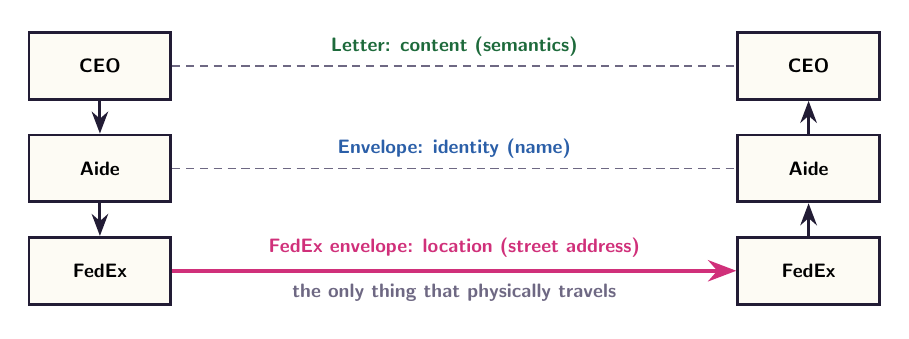
\begin{tikzpicture}[x=1cm,y=1cm,
  who/.style={blk,minimum width=1.8cm},
  pkg/.style={font=\sffamily\scriptsize\bfseries,align=center}]
  \node[who] (c1) at (0,3) {CEO};   \node[who] (c2) at (9,3) {CEO};
  \node[who] (a1) at (0,1.7) {Aide};  \node[who] (a2) at (9,1.7) {Aide};
  \node[who] (f1) at (0,0.4) {FedEx}; \node[who] (f2) at (9,0.4) {FedEx};
  \draw[arr] (c1)--(a1); \draw[arr] (a1)--(f1);
  \draw[arr] (f2)--(a2); \draw[arr] (a2)--(c2);
  \draw[arr,ppink,line width=1.6pt] (f1.east)--(f2.west);
  \draw[densely dashed,muted] (c1.east)--(c2.west) node[pkg,midway,above,text=pgreen] {Letter: \emph{content} (semantics)};
  \draw[densely dashed,muted] (a1.east)--(a2.west) node[pkg,midway,above,text=pcyan] {Envelope: \emph{identity} (name)};
  \node[pkg,text=ppink,above] at (4.5,0.45) {FedEx envelope: \emph{location} (street address)};
  \node[pkg,text=muted,below] at (4.5,0.35) {the only thing that physically travels};
\end{tikzpicture}
\figcap{The path of the letter (slide 10). Each dashed line joins two \emph{peers} that understand the same thing. The real movement goes down
on the left, across at the bottom, and up on the right.}
\end{center}

\begin{intuition}[Three lessons of the letter]
\begin{itemize}
  \item \textbf{Peers understand the same things, and no one else does.} The FedEx driver never reads the letter; the CEO never reads the street address.
  \item \textbf{Each layer adds its own wrapping}, so the lowest layer carries the most packaging.
  \item \textbf{Each layer only talks to its neighbours}: the CEO deals with the aide, never with the truck.
\end{itemize}
\end{intuition}

\subsection{The resulting five layers}

Each task becomes a layer. Two tasks are folded into the layer above them.

\begin{center}
\renewcommand{\arraystretch}{1.25}
\begin{tabular}{>{\columncolor{border}}l L{4.2cm} L{5.6cm}}
\thd{LAYER} & \cellcolor{border}\thd{TASK} & \cellcolor{border}\thd{WHAT IT IS ABOUT}\\
\rowcolor{surface} \cellcolor{border}\color{surface}5 Application & do something with the data & web, e-mail, video, games\\
\rowcolor{surface2} \cellcolor{border}\color{surface}4 Transport & ensure the packets get there & between \emph{processes}; reliability\\
\rowcolor{surface} \cellcolor{border}\color{surface}3 Network & deliver across many LANs & \textbf{global} addresses; routing\\
\rowcolor{surface2} \cellcolor{border}\color{surface}2 (Data) Link & deliver across one LAN (incl.\ packets on wire) & \textbf{local} addresses; sharing the medium\\
\rowcolor{surface} \cellcolor{border}\color{surface}1 Physical & bits on the wire (incl.\ electrons) & voltages, light, radio\\
\end{tabular}
\end{center}

\begin{intuition}[A mnemonic for the five]
Read from the bottom: \textbf{P}hysical, \textbf{L}ink, \textbf{N}etwork, \textbf{T}ransport, \textbf{A}pplication. Each layer answers one question:
\emph{how is a bit sent? to which neighbour? to which machine in the world? to which program on it? and what does the program do with it?}
\end{intuition}

\subsection{Who implements which layers?}

\slidefig{0.62\linewidth}{layers_physical}
\figcap{Slides 13--15. Host A and Host B implement all five layers; the router in the middle implements only the bottom three. The blue line is the
\emph{physical} path of the data: down Host A's stack, across the wire, up to the router's network layer, down again, and up Host B's stack.}

\begin{formula}[The top two layers live only at the hosts]
Routers implement \textbf{physical, link and network}. \textbf{Transport and application are implemented only at the end hosts}.
Inside the network, nobody looks at the transport or application data. (This is the answer to the second design question of \S1.1: \emph{where} each module is implemented.)
\end{formula}

\begin{defn}[Logical vs.\ physical communication]
\begin{itemize}
  \item \term{Logical communication}: each layer behaves as if it talks directly to its \term{peer}, the same layer on the other machine.
        Host A's transport layer ``talks to'' Host B's transport layer. The router's network layer ``talks to'' both hosts' network layers.
  \item \term{Physical communication}: the bits really go \emph{down} to the physical layer, travel peer to peer across each link, and go back \emph{up} to the relevant layer.
\end{itemize}
\end{defn}

\section{Protocols}

\begin{defn}[Protocol]
A \term{protocol} is an \textbf{agreement on how to communicate}: to exchange data, and to coordinate the sharing of resources. A protocol specifies:
\begin{itemize}
  \item its \term{syntax}: how the protocol is structured, meaning the format of the messages and the order in which they are sent and received;
  \item its \term{semantics}: what the bits mean, meaning how to respond to each message or event.
\end{itemize}
\end{defn}

\begin{example}[Protocols in life]
\begin{itemize}
  \item \textbf{Asking a question in class}: raise a hand, wait to be called on, then speak.
  \item \textbf{Turn-taking in conversation}: a pause is the signal that the next person may respond.
  \item \textbf{Boarding and leaving an airplane}: by rows or zones. Not all countries use the same protocol!
  \item \textbf{Answering the phone}: you say ``hello'' as the signal for the caller to talk; the caller identifies themselves, and then the conversation starts.
\end{itemize}
Each one has syntax (what is said, in what order) and semantics (what each signal means and what to do next).
\end{example}

\begin{example}[HTTP, an application-layer protocol]
A browser asks a web server for a page. The request (syntax: a method, a path, a version, then header lines, then an empty line):
\begin{center}\begin{minipage}{0.8\linewidth}\ttfamily\footnotesize
GET /courses/archive/spring06/cos461/ HTTP/1.1\\
Host: www.cs.princeton.edu\\
User-Agent: Mozilla/4.03\\
\textit{(empty line)}
\end{minipage}\end{center}
The response (semantics: \texttt{200 OK} means ``here it is''):
\begin{center}\begin{minipage}{0.8\linewidth}\ttfamily\footnotesize
HTTP/1.1 200 OK\\
Date: Mon, 6 Feb 2006 13:09:03 GMT\\
Server: Netscape-Enterprise/3.5.1\\
Last-Modified: Mon, 6 Feb 2006 11:12:23 GMT\\
Content-Length: 21\\
\textit{(empty line)}\\
Site under construction
\end{minipage}\end{center}
\texttt{Content-Length: 21} tells the browser exactly how many bytes of body to read: ``Site under construction'' is 23 characters, so the slide's
example is slightly off, but the idea is that the header announces the length.
\end{example}

\begin{example}[IP, a network-layer protocol]
Lower layers use binary formats with fixed-size fields. The IP packet header:
\slidefig{0.62\linewidth}{ip_header}
\figcap{Slide 20. Each row is 32 bits. Without options the header is 5 rows $=20$ bytes. The fields you need now: \emph{Version} (4 for IPv4),
\emph{Total Length}, \emph{Time to Live} (decremented by each router; the packet is dropped at 0), \emph{Protocol} (which transport protocol is inside, e.g.\ TCP),
and the 32-bit \emph{source} and \emph{destination} addresses.}
\end{example}

\subsection{Standardization}

\begin{intuition}[Why standards]
Everyone must follow the same protocol. Very small changes can make a big difference, or stop communication altogether: if one side thinks the
length field is 16 bits and the other 32, nothing works. Hence \textbf{standards}. A standard fixes the protocol, \emph{not} the code, so there can be many
independent implementations (Windows, Linux and macOS each have their own TCP).
\end{intuition}

\begin{defn}[IETF and RFCs]
The \term{Internet Engineering Task Force} (IETF, \texttt{ietf.org}) writes the Internet's standards. It works in \emph{working groups} focused on specific
issues, and publishes its documents as numbered \term{Requests For Comments} (RFCs), archived at \texttt{rfc-editor.org}. (Link-layer standards such as Ethernet and WiFi come from the IEEE 802 committees.)
\end{defn}

\subsection{The Internet protocol suite, end to end}

\slidefig{0.82\linewidth}{ip_suite}
\figcap{Slide 22. Each layer's unit of data has its own name: the application sends an \emph{HTTP message}, the transport layer a \emph{TCP segment},
the network layer an \emph{IP packet} (datagram), and the link layer a \emph{frame}. The two routers process only IP and below. Notice that the link changes along the way: Ethernet, then SONET, then Ethernet again. IP runs over all of them.}

\subsection{Encapsulation}

\begin{defn}[Encapsulation]
Going down the stack, each layer takes what it received from above as its \emph{payload} and adds its own \emph{header} in front.
This is \term{encapsulation}. Going up the stack at the receiver, each layer removes its own header and passes the payload up (\term{decapsulation}).
\end{defn}

\slidefig{0.72\linewidth}{encapsulation}
\figcap{Slide 23. User A's request ``Get index.html'' (green) gets a transport header (connection ID), then a network header (source and destination
addresses), then a link header (local source and destination). At User B the headers are removed in the opposite order.}

\textbf{Step by step for one web request} \src{KR 1.5.2}:
\begin{enumerate}
  \item The application builds the HTTP message $M$.
  \item Transport adds a header $H_t$ (which process on which host): segment $=H_t\,M$.
  \item Network adds $H_n$ (global source and destination addresses): datagram $=H_n\,H_t\,M$.
  \item Link adds $H_l$ (local source and destination on this LAN): frame $=H_l\,H_n\,H_t\,M$.
  \item The physical layer sends the bits. Each router strips $H_l$, reads $H_n$, and wraps the datagram in a \emph{new} link header for the next link.
\end{enumerate}

\begin{example}[How much is overhead?]
Common case: 20 bytes TCP $+$ 20 bytes IP $+$ 14 bytes Ethernet $=$ \hl{54 bytes of headers}.
\begin{itemize}
  \item A full frame with 1460 bytes of data: $1460/(1460+54)=96.4\%$ of the bytes are useful.
  \item A single typed keystroke (1 byte of data, e.g.\ in a remote shell): $1/55=1.8\%$ useful. Mice pay heavily for headers.
\end{itemize}
\end{example}

\begin{pitfall}[54 bytes counts headers only]
The 54 bytes are the three \emph{headers}. On the wire, Ethernet also adds a 4-byte CRC \emph{trailer} after the data (and an 8-byte preamble before the frame) \src{KR 6.4.2}.
So the real per-frame overhead is a bit larger.
\end{pitfall}

\section{Characterizing the layers}

\begin{defn}[Service, interface, protocol (OSI terms)]
Every layer is described by three things:
\begin{itemize}
  \item its \term{service}: \emph{what} the layer does for the layer above;
  \item its \term{service interface}: \emph{how} the layer above accesses the service;
  \item its \term{protocol}: how the \emph{peers} on different machines communicate to provide the service. The protocol governs what happens
        \emph{between} machines, not how the layer is coded on one machine.
\end{itemize}
A layer can have \textbf{many implementations}, and this is what allows innovation.
\end{defn}

\begin{center}
\renewcommand{\arraystretch}{1.3}
\small
\begin{tabular}{>{\columncolor{border}}l L{3.6cm} L{3.4cm} L{3.4cm}}
\thd{LAYER} & \cellcolor{border}\thd{SERVICE} & \cellcolor{border}\thd{PROTOCOLS DO} & \cellcolor{border}\thd{EXAMPLES}\\
\rowcolor{surface} \cellcolor{border}\color{surface}1 Physical & move bits between two systems on \emph{one} physical link & coding of bits: voltage levels, bit duration & optical, wireless (not our focus)\\
\rowcolor{surface2} \cellcolor{border}\color{surface}2 Link & exchange \term{frames} with hosts on the same LAN, using local addresses & \term{Media Access Control} (MAC) & Ethernet, 802.11, Frame Relay, ATM\\
\rowcolor{surface} \cellcolor{border}\color{surface}3 Network & deliver packets to any destination, across many layer-2 networks, using global addresses & routing & IP (only!)\\
\rowcolor{surface2} \cellcolor{border}\color{surface}4 Transport & communication between \emph{processes}; perhaps reliability, rate adaptation & reliability, flow control, splitting large messages & TCP, UDP\\
\rowcolor{surface} \cellcolor{border}\color{surface}5 Application & any service to the end user & depends on the application & HTTP, SMTP, Skype, BitTorrent\\
\end{tabular}
\end{center}

\begin{itemize}
  \item \textbf{Link interface}: ``send this frame to that local host''; ``deliver to me the frames addressed to me''. The link layer is not limited to a single wire: a LAN may have many hosts.
  \item \textbf{Network interface}: ``send this packet to that global destination''; ``deliver to me the packets for this host''. ``Inter-network'' means across \emph{different} layer-2 networks, e.g.\ from Ethernet to 802.11.
  \item \textbf{Transport interface}: ``send this message to that process on that host''; a local process receives the messages sent to it.
        \term{Multiplexing} here means that many processes on one host share the host's network connection.
\end{itemize}

\subsection{The narrow waist}

\slidefig{0.6\linewidth}{hourglass}
\figcap{The Internet hourglass (slide 30). Many applications at the top, many link and physical technologies at the bottom, and exactly one protocol in the middle: IP.}

\begin{intuition}[Why only one network-layer protocol]
The slide asks: ``IP: why no other examples?'' Because \textbf{IP is the narrow waist}. Every application runs over IP, and IP runs over every link technology.
\begin{itemize}
  \item A new application (top) only has to work with IP, and it runs on every network.
  \item A new link technology (bottom) only has to carry IP, and every application works over it.
\end{itemize}
With $A$ applications and $L$ link technologies, a single waist needs $A+L$ adaptations instead of $A\times L$. With 100 applications and 20 links: 120 instead of 2000.
The narrow waist is what makes \hl{interoperability} possible. The price: changing IP itself is extremely hard (IPv6 has been ``coming'' for decades).
\end{intuition}

\begin{pitfall}[``Waste'' vs.\ ``waist'']
Slide 30's title says ``The Narrow \emph{Waste} of the Internet''. The word is \textbf{waist}, as in the narrow middle of an hourglass, which is what the figure shows.
\end{pitfall}

\section{Building the Internet bottom up: the link layer}

The course now builds the Internet from the bottom. \textbf{Challenge I: communicating within a LAN.} For now we look only at the physical and link layers
(the physical layer itself is not the focus of the course). Transport and network come later; the link layer is needed to interconnect LANs.

\subsection{Terminology}

\begin{defn}[Node, link, frame]
\begin{itemize}
  \item \term{Nodes}: end hosts \emph{and} relays (routers, switches): anything that runs a link layer.
  \item \term{Links}: the communication channels that connect \emph{adjacent} nodes along the path. They can be wired, wireless, or logical (a broadcast domain).
  \item \term{Frame}: the layer-2 packet. It \emph{encapsulates} a network-layer datagram.
\end{itemize}
The \textbf{data-link layer} is responsible for transferring a datagram from one node to an \emph{adjacent} node over one link.
\end{defn}

\begin{example}[The trip from Honolulu to Jerusalem \src{KR 6.1}]
A taxi from Honolulu to HNL airport, a plane to Newark (EWR), a plane to Tel Aviv (TLV), a train to Jerusalem.
\begin{center}
\renewcommand{\arraystretch}{1.2}
\begin{tabular}{>{\columncolor{border}}l l}
\thd{TRAVEL} & \cellcolor{border}\thd{NETWORK}\\
\rowcolor{surface} \cellcolor{border}\color{surface}passenger & datagram\\
\rowcolor{surface2} \cellcolor{border}\color{surface}each segment of the trip & one link\\
\rowcolor{surface} \cellcolor{border}\color{surface}transportation mode (taxi, plane, train) & link-layer protocol\\
\rowcolor{surface2} \cellcolor{border}\color{surface}travel agent who plans the route & routing algorithm\\
\end{tabular}
\end{center}
The datagram crosses different links with \emph{different} link protocols (Ethernet on the first link, 802.11 on the next), and each one provides different
services. A taxi does not promise what a plane does, and some links are reliable while others are not.
\end{example}

\subsection{Services of a single link}

\begin{itemize}
  \item \textbf{Link access and addressing.} When the channel is a shared medium, someone must decide who sends. \term{MAC addresses} in the frame header
        identify the source and the destination. \hl{They are different from IP addresses} (\S\ref{sec:mac}).
  \item \textbf{Reliable delivery between adjacent nodes} (error detection and correction, retransmissions). It is seldom used on low-bit-error links (fibre, some twisted pair), but needed on wireless links, which have high error rates. This is revisited later in the course.
  \item ``\dots?'': the slide leaves the list open. \src{KR 6.1.1} also lists \emph{framing} (wrapping the datagram) and \emph{error detection} as separate services.
\end{itemize}

\subsection{Where is the link layer implemented?}

\slidefig{0.5\linewidth}{nic}
\figcap{Slide 39. Inside a host, application, transport and network run in software on the CPU. Link and physical are in the \emph{network adapter}.}

\begin{defn}[Network interface card (NIC)]
The link layer runs \textbf{in every host}, in an \term{adapter}, also called a \term{network interface card} (NIC): e.g.\ an Ethernet card or an 802.11 card.
The NIC implements the link and physical layers. It attaches to the host's system bus and is a combination of hardware, software and firmware.
\end{defn}

\begin{formula}[Adapters communicating]
\begin{itemize}
  \item \textbf{Sending side}: encapsulates the datagram in a frame and adds error-checking bits (and, if used, reliable-delivery machinery).
  \item \textbf{Receiving side}: checks for errors, extracts the datagram and passes it up to the network layer.
\end{itemize}
\end{formula}

\section{The multiple access problem}

\begin{defn}[Broadcast channel and collision]
On a \term{single shared broadcast channel}, every frame sent by one node is received by all the others. If a node receives two or more signals at the
same time, there is a \term{collision}: the signals are tangled together and \hl{all the colliding frames are lost}, and the channel was wasted during the collision \src{KR 6.3}.
\end{defn}

\begin{defn}[Multiple access protocol]
A \term{multiple access protocol} (MAC protocol) is a \textbf{distributed algorithm} that determines how the nodes share the channel, i.e.\ \emph{when} each node may transmit.
The catch: the communication about how to share the channel \hl{must use the channel itself}. There is no separate ``out-of-band'' channel for coordination.
\end{defn}

\subsection{Broadcast domains: wired}

\slidefig{0.55\linewidth}{bus_star}
\figcap{Slides 42, 96. Left: a \emph{bus}, one coaxial cable shared by every node. Right: a \emph{star}, every node on its own cable to a switch.}

\begin{itemize}
  \item \textbf{Bus} (popular until the mid-1990s): all nodes are in the same \term{collision domain}: any two of them can collide.
  \item \textbf{Star} (today): an \emph{active switch} sits in the centre. Each node runs a separate Ethernet with the switch, so \hl{nodes do not collide with each other}. Switches come later in the course.
\end{itemize}

\begin{pitfall}[Collision domain vs.\ broadcast domain]
Slide 42 says the bus nodes are in the same ``collision domain''; slide 96, the same slide repeated, says ``broadcast domain''. On a bus the two coincide, so both are true.
In general they are different things: a \emph{collision domain} is the set of nodes whose transmissions can collide; a \emph{broadcast domain} is the set
of nodes that receive a broadcast frame. The switched star still has one broadcast domain, but each cable is its own collision domain.
\end{pitfall}

\subsection{Broadcast domains: wireless}

\slidefig{0.62\linewidth}{wireless_hidden}
\figcap{Slide 43. Left: A and C are separated by a mountain; both reach B, but they cannot hear each other. Right: A's signal (red) fades with distance;
so does C's (blue). At B both are strong enough; at A, C's signal is too weak to sense, and vice versa.}

\begin{defn}[Hidden terminal and fading \src{KR 7.2}]
In wireless, ``everyone hears everyone'' is not true.
\begin{itemize}
  \item \term{Hidden terminal problem}: A and C both reach B, but an obstacle hides them from each other. Neither can tell that the other is transmitting, so they collide at B.
  \item \term{Fading}: signal strength decreases with distance. Even without an obstacle, A and C may be too far apart to hear each other, although B, in the middle, hears both.
\end{itemize}
\end{defn}

\subsection{The ideal multiple access protocol}

\begin{formula}[Wish list for a broadcast channel of rate $R$ bit/s]
\begin{enumerate}
  \item When \textbf{one} node wants to transmit, it can send at rate $R$.
  \item When $M$ nodes want to transmit, each can send at \textbf{average} rate $R/M$.
  \item \textbf{Fully decentralized}: no special node coordinates (no single point of failure).
  \item \textbf{No synchronization} of clocks or slots.
  \item \textbf{Simple}.
\end{enumerate}
\end{formula}

Keep this list in mind: every protocol below is scored against it in \S\ref{sec:scorecard}.

\subsection{A taxonomy of MAC protocols}

\begin{center}
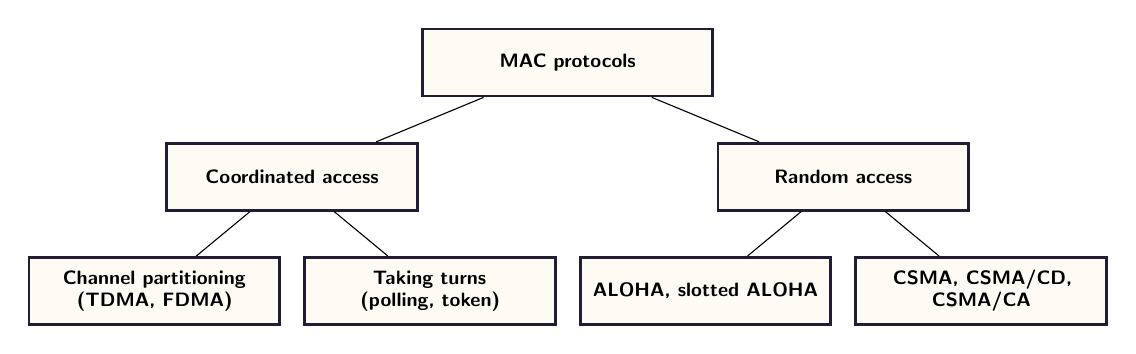
\begin{tikzpicture}[level distance=1.45cm,
  level 1/.style={sibling distance=7cm},
  level 2/.style={sibling distance=3.5cm},
  every node/.style={blk,text width=2.9cm}]
\node[text width=3.4cm] {MAC protocols}
  child {node {Coordinated access}
    child {node {Channel partitioning\\(TDMA, FDMA)}}
    child {node {Taking turns\\(polling, token)}}}
  child {node {Random access}
    child {node {ALOHA, slotted ALOHA}}
    child {node {CSMA, CSMA/CD, CSMA/CA}}};
\end{tikzpicture}
\figcap{The lecture's two broad classes (slides 45, 89, 103).}
\end{center}

\begin{itemize}
  \item \term{Channel partitioning}: divide the channel into smaller ``pieces'' (time slots or frequencies) and give each node a piece for its exclusive use.
  \item \term{Taking turns}: nodes take turns, but nodes with more to send can take longer turns.
  \item \term{Random access}: the channel is not divided. Collisions are allowed, and the protocol \emph{recovers} from them.
\end{itemize}

\begin{pitfall}[Is channel partitioning ``centralized''?]
The slides group channel partitioning under ``Centralized Coordination''. Once the slots or bands are assigned, TDMA and FDMA need \emph{no} coordinator at run time:
every node simply uses its own piece. What they need is an \emph{agreement made in advance}. Only some taking-turns protocols (polling) have a real central master.
That is why \src{KR 6.3} lists \textbf{three} classes side by side: channel partitioning, random access and taking turns. Also, slide 103 writes ``time/frequency
\emph{modulation}''. It should be time/frequency \textbf{division} (multiplexing). Modulation is how bits are put on a signal, a physical-layer matter.
\end{pitfall}

\section{Channel partitioning: TDMA and FDMA}

\begin{defn}[TDMA: time division multiple access]
Access to the channel goes in \textbf{rounds} (frames). Each station gets a fixed-length slot in every round; the slot length is one packet transmission time.
\hl{Unused slots go idle.}
\end{defn}

\begin{center}
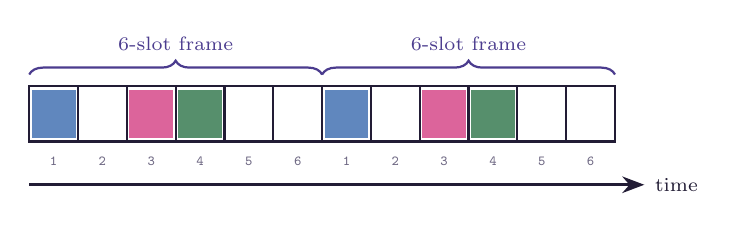
\begin{tikzpicture}[x=0.62cm,y=1cm]
  \foreach \r in {0,6} {
    \foreach \s in {1,...,6} {
      \pgfmathtruncatemacro{\x}{\r+\s-1}
      \draw[ink,line width=0.8pt] (\x,0) rectangle (\x+1,0.7);
      \node[font=\ttfamily\tiny,text=muted] at (\x+0.5,-0.25) {\s};
    }
    \draw[decorate,decoration={brace,amplitude=5pt},thick,border] (\r,0.85)--(\r+6,0.85) node[midway,above=5pt,font=\scriptsize] {6-slot frame};
  }
  \foreach \x/\c in {0/pcyan,2/ppink,3/pgreen,6/pcyan,8/ppink,9/pgreen}
    \fill[\c!75] (\x+0.05,0.05) rectangle (\x+0.95,0.65);
  \draw[arr] (0,-0.55)--(12.6,-0.55) node[right,font=\scriptsize] {time};
\end{tikzpicture}
\figcap{Slide 46's example: a 6-station LAN in which stations 1, 3 and 4 have packets. Slots 2, 5 and 6 stay idle in every frame, even though 1, 3 and 4 have more to send.}
\end{center}

\begin{defn}[FDMA: frequency division multiple access]
The channel's spectrum is divided into frequency bands, and each station is assigned a fixed band. Unused transmission time in a band goes idle.
\end{defn}

\slidefig{0.5\linewidth}{fdma}
\figcap{Slide 47. One FDM cable carries six bands. Stations 1, 3, 4 send in their bands; bands 2, 5, 6 are idle.}

\begin{example}[The cost of partitioning, with numbers \src{KR 6.3.1}]
A channel of $R=60$\,Mbps shared by $N=6$ stations: each one gets exactly $R/N=10$\,Mbps.
\begin{itemize}
  \item 6 stations busy: each gets 10\,Mbps $=R/M$. Property 2 is met perfectly, and there are no collisions.
  \item Only station 1 busy: it still gets only 10\,Mbps, and \hl{50\,Mbps are wasted}. Property 1 fails.
  \item Even when alone, a TDMA station must wait for its own slot: on average half a frame of delay before each packet.
\end{itemize}
Like a pan of Kaiserschmarrn torn into six fixed portions before the guests arrive: if only one guest is hungry, they still get one sixth, and the rest goes cold.
\end{example}

\section{Random access protocols}

\begin{defn}[Random access]
When a node has a packet to send, it transmits at the \textbf{full channel rate} $R$, with no prior coordination among the nodes.
If two or more nodes transmit, there is a \term{collision}. A random access MAC protocol specifies:
\begin{itemize}
  \item how to \textbf{detect} collisions;
  \item how to \textbf{recover} from them, e.g.\ by delayed retransmission.
\end{itemize}
Examples: slotted ALOHA, (pure) ALOHA, CSMA, CSMA/CD, CSMA/CA.
\end{defn}

\begin{intuition}[Why the delay must be random]
If two colliding nodes both waited the \emph{same} fixed time and tried again, they would collide again, forever. Each node chooses its delay
\emph{independently at random}, so with luck one of them goes first and gets through \src{KR 6.3.2}.
\end{intuition}

\section{Probability toolkit (recap of slides 49--67)}

The lecture now pauses for ``Probability 101'': sample spaces, events, probability functions, conditional probability, Bayes, random variables,
expectation, the four discrete distributions, and Examples I--III. \textbf{Week 01 Part B covers all of these in full}, including Example II (good and bad packets)
and Example III (the chain of links). Here are only the facts that the MAC analysis below uses.

\begin{formula}[What we need]
\begin{itemize}
  \item \textbf{Independent events multiply}: $P(A\cap B)=P(A)P(B)$. So ``$N-1$ independent nodes all stay silent, each with probability $1-p$'' has probability $(1-p)^{N-1}$.
  \item \textbf{Disjoint events add}: $P(A\cup B)=P(A)+P(B)$.
  \item \textbf{Exactly one success among $N$}: $\binom N1p(1-p)^{N-1}=Np(1-p)^{N-1}$, the binomial probability $P(X=1)$ for $X\sim\text{Bin}(N,p)$.
  \item \textbf{Geometric}: if each try succeeds with probability $q$, the number of tries is $\text{Geo}(q)$, with mean $1/q$. The expected number of \emph{failures} before the success is $1/q-1=(1-q)/q$.
\end{itemize}
\end{formula}

\begin{example}[Example I from the slides: 50 components]
Communication uses 50 components, each working 99\% of the time (independently). Failure probability $=1-0.99^{50}\approx39.5\%$.
With 99.9\%: $1-0.999^{50}\approx4.9\%$. \hl{The system must be designed to expect failure.}
\end{example}

\begin{pitfall}[Slide 67: ``the probability to success drops to $(1-p)$'']
In Example III (Week 01, Question 3) the success probability goes from $(1-p)^n$ to $(1-p)$. Since $1-p>(1-p)^n$ for $n\ge2$, it \textbf{rises}, not ``drops''.
Also, the slide's $\E X=1/(1-p)$ counts the sends needed to cross \emph{one} hop. Crossing all $n$ hops hop by hop takes $n/(1-p)$ link transmissions on average.
\end{pitfall}

\subsection{The new tool: $(1-1/N)^{N}\to 1/e$}

The efficiency of ALOHA ends with ``take the limit as $N\to\infty$''. This is the limit it needs.

\begin{formula}[A famous limit]
\[ \lim_{N\to\infty}\Big(1-\frac1N\Big)^{N}=\frac1e\approx0.368, \qquad\text{and therefore also}\qquad \lim_{N\to\infty}\Big(1-\frac1N\Big)^{N-1}=\frac1e. \]
(The second follows from the first: $(1-\frac1N)^{N-1}=(1-\frac1N)^{N}\big/(1-\frac1N)$, and the denominator tends to 1.)
\end{formula}

\begin{example}[See it converge]
\begin{center}
\renewcommand{\arraystretch}{1.2}
\begin{tabular}{>{\columncolor{border}}c c c}
\thd{$N$} & \cellcolor{border}\thd{$(1-1/N)^{N}$} & \cellcolor{border}\thd{$(1-1/N)^{N-1}$}\\
\rowcolor{surface} \cellcolor{border}\color{surface}2 & 0.250 & 0.500\\
\rowcolor{surface2} \cellcolor{border}\color{surface}5 & 0.328 & 0.410\\
\rowcolor{surface} \cellcolor{border}\color{surface}10 & 0.349 & 0.387\\
\rowcolor{surface2} \cellcolor{border}\color{surface}100 & 0.366 & 0.370\\
\rowcolor{surface} \cellcolor{border}\color{surface}$\infty$ & 0.368 & 0.368\\
\end{tabular}
\end{center}
Why it is true, in words: $\ln(1-x)\approx-x$ for small $x$, so $N\ln(1-\frac1N)\approx N\cdot(-\frac1N)=-1$, and $(1-\frac1N)^N\approx e^{-1}$.
In probability terms: if each of $N$ nodes stays silent with probability $1-\frac1N$, then the chance that \emph{all} stay silent tends to $1/e$. It is the Poisson probability $P(X=0)$ for mean $1$.
\end{example}

\section{Slotted ALOHA}

\begin{defn}[Slotted ALOHA]
\textbf{Assumptions}: all frames have the same size; time is divided into equal slots, each the time to transmit one frame; nodes start transmitting
only at the beginning of a slot; nodes are synchronized; if two or more nodes transmit in a slot, all nodes detect the collision.

\textbf{Operation}:
\begin{enumerate}
  \item When a node gets a fresh frame, it transmits in the next slot.
  \item No collision: success; the node may send a new frame in the next slot.
  \item Collision: the node retransmits the frame in \emph{each subsequent slot with probability $p$}, until it succeeds.
\end{enumerate}
``With probability $p$'': before each slot the node tosses a biased coin, and transmits on heads (probability $p$).
\end{defn}

\begin{center}
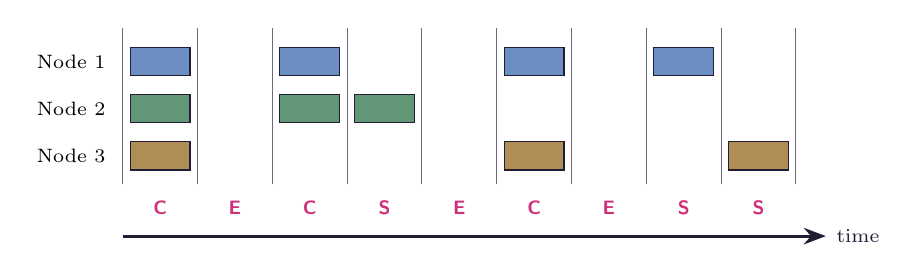
\begin{tikzpicture}[x=0.95cm,y=0.6cm]
  \foreach \i/\l in {1/C,2/E,3/C,4/S,5/E,6/C,7/E,8/S,9/S} {
    \draw[muted,thin] (\i-1,0) -- (\i-1,3.3);
    \node[font=\sffamily\scriptsize\bfseries,text=ppink] at (\i-0.5,-0.5) {\l};
  }
  \draw[muted,thin] (9,0)--(9,3.3);
  \foreach \y/\n in {2.6/1,1.6/2,0.6/3} \node[font=\scriptsize,anchor=east] at (-0.1,\y) {Node \n};
  \foreach \x/\y/\c in {0/2.6/pcyan,0/1.6/pgreen,0/0.6/pgold, 2/2.6/pcyan,2/1.6/pgreen, 3/1.6/pgreen, 5/2.6/pcyan,5/0.6/pgold, 7/2.6/pcyan, 8/0.6/pgold}
    \fill[\c!70,draw=ink] (\x+0.1,\y-0.3) rectangle (\x+0.9,\y+0.3);
  \draw[arr] (0,-1.1)--(9.4,-1.1) node[right,font=\scriptsize] {time};
\end{tikzpicture}
\figcap{Slotted ALOHA in action \src{KR Fig.\ 6.10}. C = collision, E = empty, S = success. All three nodes collide in slot 1. Node 2 succeeds in slot 4, node 1 in slot 8 and node 3 in slot 9.}
\end{center}

\textbf{Pros}: a single active node can transmit continuously at the full rate $R$; highly decentralized (only the slot times must be in sync); simple.\\
\textbf{Cons}: collisions waste slots; idle slots are wasted too; a node may detect a collision long before the slot ends but still wastes the whole slot; it needs clock synchronization.

\subsection{Goodput vs.\ throughput}

\begin{defn}[Goodput and throughput]
Consider many nodes, all with many frames to send.
\begin{itemize}
  \item \term{Goodput} (also \term{efficiency}): the long-run fraction of \emph{successful} slots.
  \item \term{Throughput}: the long-run fraction of slots in which there was a transmission, successful or not.
\end{itemize}
Throughput counts collisions as ``busy''; goodput counts only useful work. A channel full of collisions has high throughput and zero goodput.
\end{defn}

\subsection{The goodput of slotted ALOHA, step by step}

\textbf{Simplified model.} $N$ nodes, each always has a frame, and in each slot \emph{each} node transmits with probability $p$, independently
(this treats fresh frames and retransmissions alike).

\begin{enumerate}
  \item \textbf{A given node succeeds} in a slot iff it transmits \emph{and} the other $N-1$ do not. By independence:
        \[ P(\text{node $i$ succeeds})=p\,(1-p)^{N-1}. \]
  \item \textbf{Some node succeeds}: the events ``node $i$ succeeds'' for $i=1,\dots,N$ are \emph{disjoint} (two nodes cannot both succeed in one slot), so we add:
        \[ \alpha(p)=N\,p\,(1-p)^{N-1}. \]
  \item \textbf{Best $p$}: differentiate and set to zero (slide 84):
        \[ \frac{d\alpha}{dp}=N(1-p)^{N-1}-pN(N-1)(1-p)^{N-2}=N(1-p)^{N-2}\big[(1-p)-(N-1)p\big]=0 \;\Rightarrow\; p^*=\frac1N. \]
        Makes sense: on average exactly one node transmits per slot.
  \item \textbf{Best goodput}: $\alpha(p^*)=N\cdot\frac1N\big(1-\frac1N\big)^{N-1}=\big(1-\frac1N\big)^{N-1}$.
  \item \textbf{Many nodes}: by the limit above, $\alpha_{\max}\to\dfrac1e\approx0.37$.
\end{enumerate}

\begin{pitfall}[Slide 73: ``approx.'' $Np(1-p)^{N-1}$]
The slide calls $Np(1-p)^{N-1}$ ``approximately'' the probability that some node succeeds. Within the model it is \textbf{exact}: the $N$ success events are
disjoint, so their probabilities add with no approximation. The approximation comes only in the last step, when $(1-\frac1N)^{N-1}$ is replaced by its limit $1/e$.
\end{pitfall}

\begin{center}
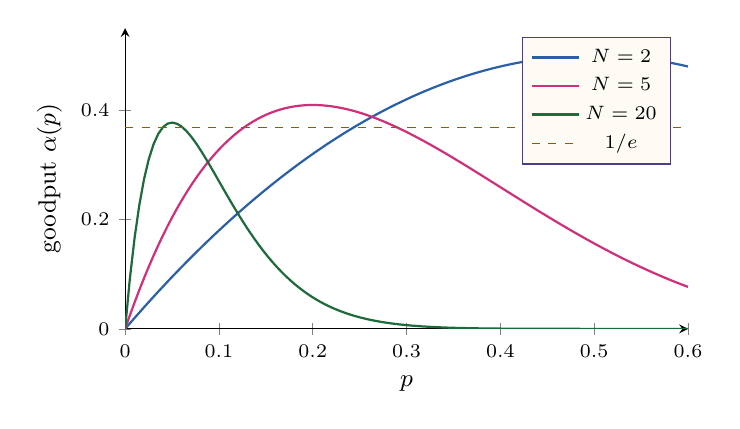
\begin{tikzpicture}
\begin{axis}[width=0.72\linewidth,height=5.4cm,xmin=0,xmax=0.6,ymin=0,ymax=0.55,
  xlabel={$p$},ylabel={goodput $\alpha(p)$},axis lines=left,
  tick label style={font=\scriptsize},label style={font=\small},
  legend style={font=\scriptsize,draw=border,fill=surface},legend pos=north east]
  \addplot[pcyan,thick,domain=0:0.6,samples=120] {2*x*(1-x)};
  \addplot[ppink,thick,domain=0:0.6,samples=120] {5*x*(1-x)^4};
  \addplot[pgreen,thick,domain=0:0.6,samples=120] {20*x*(1-x)^19};
  \addplot[pgold,dashed,domain=0:0.6] {0.3679};
  \legend{$N=2$,$N=5$,$N=20$,$1/e$}
\end{axis}
\end{tikzpicture}
\figcap{Slotted ALOHA goodput as a function of $p$. Each curve peaks at $p=1/N$; the peak heights 0.50, 0.41, 0.38 approach $1/e$.}
\end{center}

\begin{example}[Where the slots go \src{KR 6.3.2}]
With many nodes at $p=1/N$: 37\% of slots succeed, 37\% are empty ($(1-\frac1N)^N\to1/e$), and the remaining 26\% are collisions.
A 100\,Mbps slotted ALOHA LAN with many busy users delivers \hl{less than 37\,Mbps} of useful data.
\end{example}

\section{Pure (unslotted) ALOHA}

\begin{defn}[Pure ALOHA]
No slots and no synchronization: simpler. Each host behaves \emph{as if} it ran slotted ALOHA on its \emph{own} slots, sending a frame with probability $p$ in
each of them. But the other hosts' ``slots'' are not aligned with its own.
\end{defn}

\slidefig{0.55\linewidth}{pure_aloha}
\figcap{Slide 74. Node $i$'s frame (yellow) occupies $[t_0,t_0+1]$ (the frame time is the unit of time). A frame started in $[t_0-1,t_0]$ (green) overlaps its start;
a frame started in $[t_0,t_0+1]$ (purple) overlaps its end.}

\textbf{Step by step.}
\begin{enumerate}
  \item The vulnerable period is \textbf{two} frame times, $[t_0-1,t_0+1]$, instead of one.
  \item $P(\text{node $i$ succeeds})=P(\text{it transmits})\cdot P(\text{no other in }[t_0-1,t_0])\cdot P(\text{no other in }[t_0,t_0+1])=p\,(1-p)^{N-1}(1-p)^{N-1}=p\,(1-p)^{2(N-1)}.$
  \item Goodput $Np(1-p)^{2(N-1)}$. The best $p$ is $p^*=1/(2N-1)$, and as $N\to\infty$ the maximum tends to $\dfrac1{2e}\approx0.18$.
\end{enumerate}

\begin{intuition}[Half of slotted ALOHA]
Pure ALOHA's maximum is exactly half of slotted ALOHA's: $0.18$ vs.\ $0.37$. The vulnerable window is twice as long. That is the price of not synchronizing clocks.
\end{intuition}

\begin{center}
\renewcommand{\arraystretch}{1.2}
\begin{tabular}{>{\columncolor{border}}c c c}
\thd{$N$} & \cellcolor{border}\thd{SLOTTED, $(1-\frac1N)^{N-1}$} & \cellcolor{border}\thd{PURE, at $p^*=\frac1{2N-1}$}\\
\rowcolor{surface} \cellcolor{border}\color{surface}2 & 0.500 & 0.296\\
\rowcolor{surface2} \cellcolor{border}\color{surface}5 & 0.410 & 0.216\\
\rowcolor{surface} \cellcolor{border}\color{surface}20 & 0.377 & 0.191\\
\rowcolor{surface2} \cellcolor{border}\color{surface}$\infty$ & $1/e=0.368$ & $1/(2e)=0.184$\\
\end{tabular}
\end{center}

\section{CSMA: listen before you talk}

\begin{defn}[CSMA (carrier sense multiple access)]
\begin{itemize}
  \item If the channel is sensed \textbf{idle}: transmit the entire frame.
  \item If the channel is sensed \textbf{busy}: defer the transmission.
\end{itemize}
Human analogy: \emph{don't interrupt others!} ALOHA, in contrast, is the guest who keeps talking no matter who else is speaking.
\end{defn}

\subsection{Why CSMA still has collisions}

\slidefig{0.42\linewidth}{csma_collision}
\figcap{Slide 77, a \term{space-time diagram}: space horizontally (four nodes on a bus), time downwards. B starts at $t_0$; its signal (yellow) spreads in both directions. At $t_1$ B's signal has not yet reached D, so D senses an idle channel and starts too (red). The chequered area is where they collide.}

\begin{formula}[The role of propagation delay]
Carrier sensing only tells a node what was on the channel \emph{one propagation delay ago}. Two nodes may each sense ``idle'' while the other's signal is
still on its way. \hl{The longer the propagation delay between nodes, the larger the collision probability.}
In plain CSMA, when a collision happens, \textbf{the whole frame transmission time is wasted}: B and D both keep transmitting to the end.
\end{formula}

\section{CSMA/CD: collision detection}

\begin{defn}[CSMA/CD]
Carrier sensing as in CSMA, plus \term{collision detection}: a node keeps listening while it transmits. Collisions are detected within a short time, and
the colliding transmissions are \textbf{aborted}, which reduces the waste. Human analogy: the polite conversationalist who stops when someone else starts talking.
\begin{itemize}
  \item \textbf{Easy in wired LANs}: compare the signal transmitted with the signal received.
  \item \textbf{Hard in wireless LANs}: the node's own transmission overwhelms the weak signal it receives from others.
\end{itemize}
\end{defn}

\slidefig{0.42\linewidth}{csmacd_detect}
\figcap{Slide 79: the same scenario with collision detection. B and D each stop shortly after the other's signal arrives. The wasted area is much smaller than in plain CSMA.}

\begin{formula}[The CSMA/CD protocol (slide 80)]
All hosts transmit and receive on one channel. When a host has a packet to send:
\begin{enumerate}
  \item \textbf{Carrier sense}: check that the line is quiet before transmitting.
  \item \textbf{Collision detection}: detect a collision as soon as possible. If one is detected, stop transmitting, wait a random time, and return to step 1.
\end{enumerate}
\end{formula}

\subsection{The worst case: how long until a collision is detected?}

\slidefig{0.78\linewidth}{csmacd_timing}
\figcap{Slide 81. A and B are at the two ends of the cable, one propagation delay PROP apart.}

\textbf{The events, step by step} ($\varepsilon$ is a tiny time):
\begin{enumerate}
  \item $t=0$: A senses idle and starts transmitting.
  \item $t=\PROP-\varepsilon$: A's first bit has \emph{almost} reached B. B senses the line idle and starts its own packet.
  \item $t=\PROP$: A's bits reach B. B is receiving while transmitting, so \textbf{B detects the collision} (after only $\varepsilon$).
  \item B's first bits travel back to A, arriving at $t=2\,\PROP-\varepsilon$. Only now does \textbf{A detect the collision}.
\end{enumerate}

\begin{formula}[Minimum frame duration (slide 82)]
To be sure that a packet was sent without collision, a host must be able to detect a collision \textbf{before it finishes transmitting} the packet.
In the worst case detection takes almost $2\,\PROP$, so
\[ \TRANSP \;\ge\; 2\cdot\PROP . \]
If A had already finished at $t<2\,\PROP$, it would wrongly believe the packet had got through.
\end{formula}

\begin{example}[Why Ethernet waits in units of 512 bits]
Classic 10\,Mbps Ethernet uses 512 bit times as its basic unit (slide 91). At 10\,Mbps one bit takes $0.1\,\mu$s, so 512 bits take $51.2\,\mu$s.
A frame of at least 512 bits (64 bytes) therefore lasts at least $51.2\,\mu$s, which covers a round trip $2\,\PROP$ of up to $51.2\,\mu$s. At $2\times10^8$\,m/s
that is about 5\,km of round trip, so about 2.5\,km of cable end to end (in practice less, because repeaters add delay).
\end{example}

\subsection{The goodput of CSMA/CD (slides 83--88)}

\begin{defn}[Efficiency $\eta$]
\[ \eta=\frac{\text{time taken to send data}}{\text{time taken to send data}+\text{overhead}}. \]
\end{defn}

\textbf{Model.} Time is slotted, and all packets have the same length. A \textbf{slot is $2\,\PROP$}, the longest it can take to detect a collision.
In each slot, each of $N$ hosts decides to transmit with probability $p$ (first transmissions and retransmissions alike).

\begin{enumerate}
  \item \textbf{A slot is ``won''} when exactly one host transmits. As in slotted ALOHA,
        \[ \alpha(p)=\binom N1p(1-p)^{N-1}, \qquad \alpha_{\max}=\Big(1-\tfrac1N\Big)^{N-1}\ \text{at } p=\tfrac1N. \]
  \item \textbf{Wasted slots.} Let $A$ be the expected number of slots wasted before a packet gets through. In the first slot: with probability $\alpha$ we win and waste $0$;
        with probability $1-\alpha$ we waste this slot and are back where we started, still expecting $A$ more:
        \[ A=\alpha\cdot0+(1-\alpha)(1+A)\quad\Rightarrow\quad A=\frac{1-\alpha}{\alpha}. \]
        This is exactly ``failures before the first success'' of a geometric variable.
  \item \textbf{With $\alpha=0.4$}: $A=0.6/0.4=1.5$. Coin check (slide 85): a coin with $P(\text{heads})=0.4$ needs on average $1/0.4=2.5$ tosses, i.e.\ 1.5 failures and then 1 success.
  \item \textbf{Efficiency.} Each packet costs its transmission time plus $A$ wasted slots of $2\,\PROP$:
        \[ \eta_{\text{CSMA/CD}}=\frac{\TRANSP}{\TRANSP+A\cdot2\,\PROP}=\frac{\TRANSP}{\TRANSP+3\,\PROP}=\frac{1}{1+3a},\qquad a\equiv\frac{\PROP}{\TRANSP}. \]
  \item \textbf{More precise models and simulation} give $\eta_{\text{CSMA/CD}}\approx\dfrac{1}{1+5a}$.
\end{enumerate}

\begin{pitfall}[Slide 84: ``$\alpha_{\max}\approx37\%\approx40\%$'']
37\% and 40\% are not the same number. $\alpha_{\max}=(1-\frac1N)^{N-1}$ is 41\% for $N=5$ and falls to $1/e=37\%$ only as $N\to\infty$. The slides then round to $\alpha=0.4$ to get the neat $A=1.5$.
With the large-$N$ value $\alpha=1/e$ we get $A=e-1\approx1.72$ and $\eta=1/(1+3.44a)$. The message is the same: the overhead is a small multiple of PROP per packet.
\end{pitfall}

\begin{intuition}[Everything depends on $a=\PROP/\TRANSP$]
$a$ compares ``how long it takes to find out about a collision'' with ``how long the useful work lasts''.
\begin{itemize}
  \item $a\to0$ (short cable or long frames): $\eta\to1$. A collision is noticed and aborted almost instantly.
  \item $a$ large (long distances, very fast links, short frames): $\eta$ collapses. This is why CSMA/CD only works in a \emph{local} area.
\end{itemize}
\end{intuition}

\begin{center}
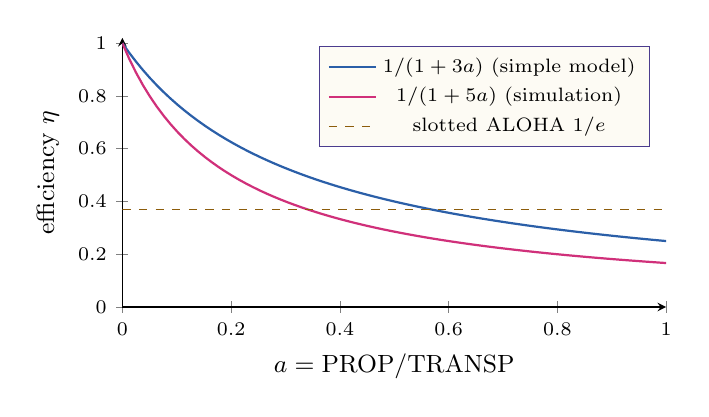
\begin{tikzpicture}
\begin{axis}[width=0.7\linewidth,height=5cm,xmin=0,xmax=1,ymin=0,ymax=1.02,
  xlabel={$a=\PROP/\TRANSP$},ylabel={efficiency $\eta$},axis lines=left,
  tick label style={font=\scriptsize},label style={font=\small},
  legend style={font=\scriptsize,draw=border,fill=surface},legend pos=north east]
  \addplot[pcyan,thick,domain=0:1,samples=80] {1/(1+3*x)};
  \addplot[ppink,thick,domain=0:1,samples=80] {1/(1+5*x)};
  \addplot[pgold,dashed,domain=0:1] {0.3679};
  \legend{$1/(1+3a)$ (simple model),$1/(1+5a)$ (simulation),slotted ALOHA $1/e$}
\end{axis}
\end{tikzpicture}
\figcap{CSMA/CD efficiency vs.\ $a$. For a LAN, $a$ is around $0.01$, so $\eta$ is above 90\%, far better than ALOHA's 37\%.}
\end{center}

\section{Summary of MAC protocols}

\begin{itemize}
  \item \textbf{Channel partitioning} by time, frequency or code: TDMA, FDMA (and CDMA).
  \item \textbf{Taking turns}:
    \begin{itemize}
      \item \term{polling} from a central site: a master node invites each node in turn to send up to some maximum number of frames;
      \item \term{token passing}: a special ``token'' frame is passed from node to node, and only the holder may send.
    \end{itemize}
    Examples: Bluetooth, FDDI, IBM Token Ring \src{KR 6.3.3}.
  \item \textbf{Random access}: ALOHA, slotted ALOHA, CSMA, CSMA/CD. Carrier sensing is easy in some technologies (wire) and hard in others (wireless).
        \hl{CSMA/CD is used in Ethernet; CSMA/CA in 802.11 (WiFi).}
\end{itemize}

\subsection{Scorecard against the wish list}\label{sec:scorecard}

\begin{center}
\renewcommand{\arraystretch}{1.25}
\small
\begin{tabular}{>{\columncolor{border}}l c c c c c}
\thd{PROTOCOL} & \cellcolor{border}\thd{1: ALONE $\to R$} & \cellcolor{border}\thd{2: $M$ BUSY $\to R/M$} & \cellcolor{border}\thd{3: DECENTR.} & \cellcolor{border}\thd{4: NO SYNC} & \cellcolor{border}\thd{5: SIMPLE}\\
\rowcolor{surface} \cellcolor{border}\color{surface}TDMA & no ($R/N$) & yes & yes$^*$ & no & yes\\
\rowcolor{surface2} \cellcolor{border}\color{surface}FDMA & no ($R/N$) & yes & yes$^*$ & yes & yes\\
\rowcolor{surface} \cellcolor{border}\color{surface}Polling & almost & almost & no (master) & yes & fairly\\
\rowcolor{surface2} \cellcolor{border}\color{surface}Slotted ALOHA & yes & no ($\le0.37R$) & yes & no & yes\\
\rowcolor{surface} \cellcolor{border}\color{surface}Pure ALOHA & yes & no ($\le0.18R$) & yes & yes & yes\\
\rowcolor{surface2} \cellcolor{border}\color{surface}CSMA/CD & yes & nearly ($\eta\approx\frac1{1+5a}$) & yes & yes & yes\\
\end{tabular}
\end{center}
{\small $^*$ once the slots or bands have been assigned. No protocol scores ``yes'' everywhere; random access gives up property 2 under heavy load in exchange for everything else.}

\section{Ethernet's CSMA/CD algorithm}

\begin{formula}[Ethernet CSMA/CD, as run by the NIC (slide 90)]
\begin{enumerate}
  \item The NIC receives a datagram from the network layer and creates a frame.
  \item If the NIC senses the channel \textbf{idle}, it starts transmitting the frame. If it senses the channel \textbf{busy}, it waits until the channel is idle, then transmits.
  \item If the NIC transmits the entire frame without detecting another transmission, it is done with the frame.
  \item If the NIC detects another transmission while transmitting, it \textbf{aborts} and sends a \term{jam signal}.
  \item After aborting, the NIC enters \term{binary exponential backoff}: after the $m$-th collision it chooses $K$ at random from $\{0,1,2,\dots,2^m-1\}$,
        waits $K\cdot512$ bit times, and returns to step 2.
\end{enumerate}
\end{formula}

\begin{defn}[Jam signal and bit time]
\begin{itemize}
  \item \term{Jam signal}: 48 bits sent after aborting, to make sure that \emph{all} other transmitters notice the collision.
  \item \term{Bit time}: the time to send one bit: $0.1\,\mu$s at 10\,Mbps (and $0.01\,\mu$s at 100\,Mbps).
\end{itemize}
\end{defn}

\subsection{Exponential backoff, step by step}

\textbf{Goal}: adapt the retransmission attempts to the current load. Under heavy load, the random wait should be longer.
\begin{center}
\renewcommand{\arraystretch}{1.2}
\begin{tabular}{>{\columncolor{border}}c c c c}
\thd{COLLISION $m$} & \cellcolor{border}\thd{$K$ CHOSEN FROM} & \cellcolor{border}\thd{MAX WAIT AT 10\,MBPS} & \cellcolor{border}\thd{P(2 NODES PICK SAME $K$)}\\
\rowcolor{surface} \cellcolor{border}\color{surface}1 & $\{0,1\}$ & $51.2\,\mu$s & 1/2\\
\rowcolor{surface2} \cellcolor{border}\color{surface}2 & $\{0,\dots,3\}$ & $153.6\,\mu$s & 1/4\\
\rowcolor{surface} \cellcolor{border}\color{surface}3 & $\{0,\dots,7\}$ & $358.4\,\mu$s & 1/8\\
\rowcolor{surface2} \cellcolor{border}\color{surface}10 and up & $\{0,\dots,1023\}$ & $\approx52.4$\,ms & 1/1024\\
\end{tabular}
\end{center}
\begin{itemize}
  \item The wait for $K$ is $K\cdot512\cdot0.1\,\mu$s $=K\cdot51.2\,\mu$s. For $K=1023$: $1023\times51.2\,\mu\text{s}\approx52.4$\,ms, the slide's ``about 50\,msec''.
  \item The last column is for \emph{two} colliding nodes: they collide again only if they pick the same $K$, which happens with probability $1/2^m$.
\end{itemize}

\begin{intuition}[Why ``exponential'' is the right shape \src{KR 6.3.2}]
We want the interval to be \textbf{short when few nodes collide} (so the channel is not left idle) and \textbf{long when many collide} (so their random choices spread out).
Nobody knows how many nodes are colliding, but each new collision is evidence that there are many, so the interval doubles. The doubling stops at $m=10$.
\end{intuition}

\section{MAC addresses}\label{sec:mac}

\begin{defn}[MAC address]
A \term{MAC address} (also LAN, physical or Ethernet address) is used to get a frame from one interface to another \emph{physically connected} interface on the same network.
For most LANs it is \textbf{48 bits} long, written as 6 bytes in hexadecimal, e.g.\ \texttt{1A-2F-BB-76-09-AD}. It is burned into the NIC's ROM, and is sometimes also settable in software.
\end{defn}

\slidefig{0.5\linewidth}{lan_addresses}
\figcap{Slide 94. Each adapter (blue) on the LAN has its own unique MAC address. Addresses belong to adapters, not to hosts: a host with two NICs has two MAC addresses \src{KR 6.4.1}.}

\begin{formula}[Who hands out MAC addresses]
The IEEE administers the address space. A manufacturer buys a block of addresses: the IEEE fixes the first 24 bits, and the manufacturer assigns the last 24 bits,
which is $2^{24}\approx16.8$ million unique addresses per block \src{KR 6.4.1}. In total there are $2^{48}\approx2.8\times10^{14}$ addresses.
\end{formula}

\begin{intuition}[Flat vs.\ hierarchical: ID number vs.\ postal address]
A MAC address is like your \textbf{ID number} (\emph{teudat zehut}): a \term{flat} identifier that says nothing about where you are, and stays the same wherever you go.
So a network card can be moved from one LAN to another and keep its address: \hl{flat $\Rightarrow$ portable}.
An IP address (later in the course) is \term{hierarchical}, like a postal address: it encodes \emph{where} you are, so it must change when you move, and it is not portable.
\end{intuition}

\section{Ethernet}

\slidefig{0.45\linewidth}{metcalfe}
\figcap{Bob Metcalfe's original Ethernet sketch (slide 97): stations attached through transceivers to one shared cable, ``the ether''.}

\begin{defn}[Ethernet]
The ``dominant'' wired LAN technology: cheap (about \$20 for a NIC); the first widely used LAN technology; simpler and cheaper than token LANs and ATM;
it kept up with the speed race, from 10\,Mbps to 100\,Gbps. Metcalfe created it by modifying the ALOHA protocol into CSMA/CD \src{KR 6.3.2}.
\end{defn}

\begin{formula}[Ethernet goodput (slide 98)]
Let $t_{\text{prop}}$ = the maximum propagation delay between two nodes in the LAN, and $t_{\text{trans}}$ = the time to transmit a maximum-size frame. Then
\[ \text{goodput}\approx\frac{1}{1+5\,t_{\text{prop}}/t_{\text{trans}}}. \]
Goodput tends to 1 as $t_{\text{prop}}\to0$ and as $t_{\text{trans}}\to\infty$. This is the $1/(1+5a)$ of CSMA/CD with $a=t_{\text{prop}}/t_{\text{trans}}$.
\end{formula}

\begin{example}[A 10\,Mbps Ethernet with numbers]
Maximum frame $\approx1518$ bytes $=12{,}144$ bits, so $t_{\text{trans}}=12{,}144/10^7\approx1.21$\,ms. A 500\,m cable at $2\times10^8$\,m/s: $t_{\text{prop}}=2.5\,\mu$s.
Then $a=2.5/1214\approx0.0021$ and goodput $\approx1/(1+0.0103)\approx99\%$.

Now speed the same LAN up to 1\,Gbps: $t_{\text{trans}}\approx12.1\,\mu$s, $a\approx0.21$, goodput $\approx1/(1+1.03)\approx49\%$.
\hl{Faster links shrink $t_{\text{trans}}$ and make the shared-bus design worse}, one reason today's Ethernet uses switched stars.
\end{example}

\section{WiFi (IEEE 802.11): CSMA/CA}

\begin{formula}[Why WiFi cannot use collision detection (slide 99)]
802.11 does carrier sensing (it does not start while another node is transmitting), but it has \textbf{no collision detection}:
\begin{itemize}
  \item it is hard to receive (sense a collision) while transmitting, because the received signals are weak compared to the node's own (fading);
  \item even then, it could not sense all collisions: the \textbf{hidden terminal} problem and fading mean the collision happens at the receiver, out of the sender's hearing.
\end{itemize}
So the goal changes: \textbf{avoid} collisions. Hence CSMA/C(ollision)A(voidance).
\end{formula}

\begin{defn}[802.11 CSMA/CA (slide 100)]
\textbf{Sender}:
\begin{enumerate}
  \item If it senses the channel idle for a period called \term{DIFS} (distributed inter-frame space), it transmits the entire frame (there is no CD, so there is no aborting).
  \item If it senses the channel busy, it starts a \textbf{random backoff} timer. The timer counts down only while the channel is idle (it is frozen while busy). The node transmits when the timer expires.
        If no ACK comes back, it increases the random backoff interval and repeats step 2.
\end{enumerate}
\textbf{Receiver}: if the frame is received OK, it returns an \term{ACK} after a short period \term{SIFS} (short inter-frame space).
\end{defn}

\slidefig{0.4\linewidth}{csma_ca}
\figcap{Slide 100. The sender waits DIFS, sends the data; the receiver waits SIFS and sends the ACK.}

\begin{intuition}[Why ACKs, and why back off even after an idle channel \src{KR 7.3.2}]
\begin{itemize}
  \item \textbf{ACKs}: without collision detection, the sender cannot know whether its frame arrived. Wireless links also have high bit-error rates. The link-layer ACK is the only evidence.
  \item \textbf{Backoff}: suppose two stations wait for a third to finish. With Ethernet's rule they would both start the moment it ends, and collide, which is cheap in Ethernet because they abort.
        In WiFi a collision costs the \emph{whole} frame. So both draw random backoffs instead; the one with the smaller value goes first, and the other hears it and freezes its counter.
\end{itemize}
\end{intuition}

\subsection{Reserving the channel: RTS and CTS}

\begin{defn}[RTS/CTS (slide 101)]
Idea: let the sender \textbf{reserve} the channel instead of sending long data frames at random.
\begin{enumerate}
  \item The sender first transmits a small \term{request-to-send} (RTS) packet to the access point (AP), using CSMA. RTSs may still collide with each other, but they are short, so little time is lost.
  \item The AP broadcasts a \term{clear-to-send} (CTS) in response to the RTS.
  \item \textbf{Every node hears the CTS}, including nodes hidden from the sender. The sender transmits its data frame, and the other stations defer.
\end{enumerate}
\hl{Collisions of data frames are avoided completely, using small reservation packets.}
\end{defn}

\slidefig{0.65\linewidth}{rts_cts}
\figcap{Slide 102. A and B send RTS at the same time: a \emph{reservation collision} (cheap, the RTS is short). A retries; the AP answers CTS(A), heard by both A and B.
A sends DATA(A); B defers until the ACK(A).}

\begin{example}[Why RTS/CTS solves the hidden terminal]
Take slide 43's picture: A and C are hidden from each other behind the mountain, and both reach B, the AP.
\begin{enumerate}
  \item A sends an RTS to B. C does not hear it.
  \item B broadcasts CTS(A). \textbf{C hears the CTS}, because C does reach B.
  \item C now knows the channel is reserved, and stays quiet until it hears B's ACK(A).
\end{enumerate}
Carrier sensing failed because C could not hear A, the \emph{sender}. RTS/CTS works because C can hear B, the \emph{receiver}, which is exactly where collisions happen.
\end{example}

\begin{example}[Is the reservation worth it?]
Say RTS and CTS take $20\,\mu$s each and a data frame takes $1000\,\mu$s. A data-frame collision wastes $1000\,\mu$s; an RTS collision wastes only $20\,\mu$s.
The price is about $40\,\mu$s of extra control per frame, $4\%$. It pays off when collisions are likely. It does not pay off for very short frames, where the RTS/CTS would be as long as the data.
\end{example}

\section{Summary: MAC protocols in practice}

\begin{intuition}[Week 02 in one paragraph]
Networks are built as a stack of five layers: physical, link, network, transport, application. Each layer talks only to its neighbours and its peers, and adds
its own header (encapsulation). IP is the single narrow waist. Building bottom up, the first challenge is a LAN: a shared broadcast link needs a MAC protocol.
\textbf{Channel partitioning} (TDMA, FDMA) is fair but wastes the channel when few nodes are busy. \textbf{Random access} gives a lone node the full rate but loses
to collisions: slotted ALOHA at most $1/e\approx37\%$, pure ALOHA $1/(2e)\approx18\%$. Listening first (CSMA) and aborting early (CSMA/CD, \emph{Ethernet}) push the
efficiency to $1/(1+5a)$, close to 100\% in a LAN. Wireless cannot detect collisions, so \emph{802.11} avoids them (CSMA/CA, ACKs, RTS/CTS).
\end{intuition}

% =================================================================
\parttitle{PART B \textperiodcentered\ RECITATION 2}{ALOHA, Step by Step}
% =================================================================

\begin{plainbox}
\textbf{What the recitation adds.} Recitation 2 (``ALOHA'', 50 slides, 19 October 2026) revisits the random access part of the lecture, but from the
exam's point of view. Parts of it repeat Part A (slotted and pure ALOHA). The new material is:
\begin{itemize}
  \item the 7-layer \textbf{OSI model} (the lecture used 5 layers);
  \item precise definitions of \textbf{bandwidth, throughput and goodput}, with two warm-up calculations;
  \item \textbf{two ways} to compute the goodput (one slot vs.\ waiting for a success) and the \textbf{binomial vs.\ Poisson} models;
  \item two exam-style questions that \textbf{mix} slotted and pure ALOHA in one network.
\end{itemize}
Every slide question is solved in full below, then extended with numbers. The recitation announces a Poisson analysis but never does it; \S\ref{sec:poisson} fills it in,
following Bertsekas \& Gallager \src{BG 4.2.2, 4.2.4}.
\end{plainbox}

\section{The OSI model: seven layers}

The lecture built the Internet's \emph{five} layers (Part A, \S Layering). The recitation starts from the older reference model with \emph{seven}.

\begin{defn}[OSI model]
The \term{Open Systems Interconnection (OSI) model} is an abstract description of the functions a communication system needs, split into layers.
As in Part A, \hl{each layer uses the service of the layer beneath it and serves the layer above it}. OSI has 7 layers; the Internet stack merges three of them into one and has 5.
\end{defn}

\begin{center}
\renewcommand{\arraystretch}{1.25}
\begin{tabular}{>{\columncolor{border}}c l l p{6.2cm}}
\thd{\#} & \cellcolor{border}\thd{LAYER} & \cellcolor{border}\thd{DATA UNIT} & \cellcolor{border}\thd{FUNCTION}\\
\rowcolor{surface} \cellcolor{border}\color{surface}7 & Application & data & high-level APIs between applications (e.g.\ an HTTP GET)\\
\rowcolor{surface2} \cellcolor{border}\color{surface}6 & Presentation & data & translating data between the network and the application (e.g.\ encryption, compression)\\
\rowcolor{surface} \cellcolor{border}\color{surface}5 & Session & data & managing a continuing session (setting it up, checkpointing, ending it)\\
\rowcolor{surface2} \cellcolor{border}\color{surface}4 & Transport & segment & delivery between processes, reliable or not (acknowledgements)\\
\rowcolor{surface} \cellcolor{border}\color{surface}3 & Network & packet & multi-hop networks: global addressing, routing\\
\rowcolor{surface2} \cellcolor{border}\color{surface}2 & Data link & frame & delivering frames between two neighbouring nodes\\
\rowcolor{surface} \cellcolor{border}\color{surface}1 & Physical & bit & sending raw bits over a medium (copper, fibre, air)\\
\end{tabular}
\end{center}

\begin{intuition}[Where did layers 5 and 6 go?]
The Internet stack has no separate session or presentation layer. If an application needs these services (encryption, for example, through TLS), \hl{the application provides them itself}.
That is why the Internet has 5 layers: OSI layers 5--7 together form the Internet's application layer.
\end{intuition}

\begin{example}[Which layer? (slide 6)]
DNS, HTTP $\to$ layer 7. TCP, UDP $\to$ layer 4. IP $\to$ layer 3. MAC protocols (ALOHA, CSMA/CD) $\to$ layer 2. The radio or the cable $\to$ layer 1.
\end{example}

\begin{pitfall}[Slide 6: ``Layer 1: Wi-Fi'', ``Layer 2: MAC'']
\textbf{Wi-Fi is not just a layer 1 protocol.} IEEE 802.11 specifies \emph{both} the physical layer (radio) \emph{and} the link layer, including its MAC protocol, CSMA/CA (Part A, \S WiFi).
Ethernet is likewise both layers 1 and 2. And ``MAC'' is not one protocol but a \emph{sub-layer} of layer 2: the part that decides who may transmit. ALOHA, CSMA/CD and CSMA/CA are all MAC protocols.
\end{pitfall}

\section{Random access: the setting}

\begin{defn}[Shared medium]
In a \term{shared medium}, all nodes transmit on, and listen to, the same channel. The recitation's rules:
\begin{enumerate}
  \item a node that transmits uses the \hl{full bandwidth} of the link;
  \item if two or more nodes transmit at the same time, there is a \term{collision} and \hl{all the data involved is lost};
  \item noise is ignored: a frame that does not collide arrives intact.
\end{enumerate}
\end{defn}

\begin{center}
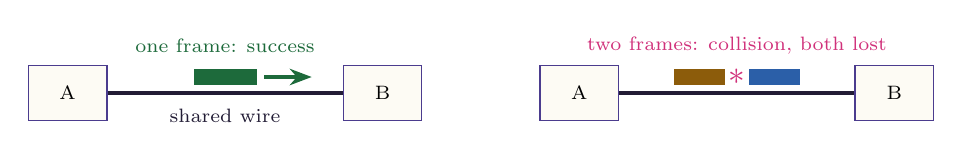
\begin{tikzpicture}[font=\scriptsize]
  \begin{scope}
    \node[draw=border,fill=surface,minimum width=1cm,minimum height=0.7cm] (a) at (0,0) {A};
    \node[draw=border,fill=surface,minimum width=1cm,minimum height=0.7cm] (b) at (4,0) {B};
    \draw[line width=1.4pt,ink] (a)--(b) node[midway,below=2pt]{shared wire};
    \fill[pgreen] (1.6,0.1) rectangle (2.4,0.3);
    \draw[arr,pgreen] (2.5,0.2)--(3.1,0.2);
    \node[pgreen] at (2,0.6) {one frame: success};
  \end{scope}
  \begin{scope}[xshift=6.5cm]
    \node[draw=border,fill=surface,minimum width=1cm,minimum height=0.7cm] (a) at (0,0) {A};
    \node[draw=border,fill=surface,minimum width=1cm,minimum height=0.7cm] (b) at (4,0) {B};
    \draw[line width=1.4pt,ink] (a)--(b);
    \fill[pgold] (1.2,0.1) rectangle (1.85,0.3);
    \fill[pcyan] (2.15,0.1) rectangle (2.8,0.3);
    \node[ppink,font=\bfseries\large] at (2,0.2) {$\ast$};
    \node[ppink] at (2,0.6) {two frames: collision, both lost};
  \end{scope}
\end{tikzpicture}
\figcap{After slide 8.}
\end{center}

\section{Bandwidth, throughput and goodput}

\begin{defn}[Bandwidth $B$]
The \term{bandwidth} $B$ is the maximum rate at which the channel can carry data, in bits per second. A frame of $L$ bits therefore takes $T = L/B$ seconds to send.
(Kurose \& Ross call the same quantity the transmission rate $R$ \src{KR 1.4.1}.)
\end{defn}

\begin{defn}[Throughput and goodput (recitation's definitions)]
\begin{itemize}
  \item \term{Throughput}: the fraction of the bandwidth (equivalently, of the time) that is used to send \emph{anything}, including frames that collide.
  \item \term{Goodput} $\eta$: the fraction of the bandwidth used to send traffic \emph{successfully}:
  \[ \eta = \frac{\text{average effective bandwidth used}}{\text{total bandwidth}} = \frac{\text{average time of successful transmissions}}{\text{total time}}, \]
  with $0\le\eta\le1$.
\end{itemize}
The two forms agree because a transmitting node always uses the full bandwidth. Here both quantities are unitless fractions.
\end{defn}

\begin{intuition}[A noisy classroom (slide 9)]
In a class where everybody talks at once, the air is busy all the time: \textbf{throughput is high}. But nobody can follow anything: \textbf{goodput is close to zero}.
A random access protocol is judged by its goodput.
\end{intuition}

\begin{pitfall}[Throughput has two meanings]
In the recitation, throughput is a unitless \emph{fraction}. In Kurose \& Ross and in most of the course, throughput is a \emph{rate} in bits/s (``the rate at which the receiver gets bits'', \src{KR 1.4.4}).
The two are linked by multiplying by $B$: a goodput of $0.37$ on a 100\,Mbps link is a useful rate of $37$\,Mbps. Always check the units in a question.
\end{pitfall}

\begin{example}[Slide 10, question 1: time to send a packet]
$B = 5$ bit/s, packet size $30$ bits. \;$T = \dfrac{|\text{packet}|}{B} = \dfrac{30\text{ bit}}{5\text{ bit/s}} = 6$\,s.
\end{example}

\begin{example}[Slide 10, question 2: bandwidth needed]
We need to send 3 packets of 30 bits within 2\,s. In total that is $90$ bits, so $B = \dfrac{3\cdot30\text{ bit}}{2\text{ s}} = 45$ bit/s.
\end{example}

\begin{example}[Extension: the same questions with real numbers]
A 1500-byte Ethernet frame ($12\,000$ bits) on a 100\,Mbps link takes $T = 12\,000/10^8 = 120\,\mu$s. Streaming 1000 such frames per second needs
$B \ge 1000\cdot12\,000 = 12$\,Mbps. With a random access protocol of goodput $\eta$, the link must be faster still: $B \ge 12/\eta$\,Mbps, i.e.\ about $32.6$\,Mbps for slotted ALOHA at its best ($\eta = 1/e$).
\end{example}

\section{ALOHA: a brief history}

ALOHAnet was Norman Abramson's radio packet network at the University of Hawaii (the slides date the project to 1968; it was described in 1970) \src{KR 6.3.2, case history}.
Laying cables between mountainous islands was impractical, so terminals scattered over the islands talked to one central host by radio, on \textbf{two frequencies}:
\begin{itemize}
  \item \textbf{downlink}, central host $\to$ terminals: only the host transmits, so there is no conflict. The host also sends an acknowledgement for every packet it received;
  \item \textbf{uplink}, terminals $\to$ host: shared by all terminals, so their packets can collide.
\end{itemize}
The designers considered dividing the uplink (multiplexing, Part A, \S TDMA/FDMA), but chose instead to let every terminal simply transmit, and retransmit after a random delay if no acknowledgement came back.
That is (pure) ALOHA, the first multiple access protocol. Its random access idea inspired Bob Metcalfe's CSMA/CD and Ethernet (Part A).

\section{The general model}

\begin{defn}[The recitation's ALOHA model (slides 16--17)]
\begin{itemize}
  \item $N$ nodes; usually we look at the limit of many nodes, $N\to\infty$.
  \item Bandwidth $B$; every frame has $L$ bits. Time is divided into \term{slots} of length $T = L/B$: \hl{one slot = the time to send one frame}.
  \item A successful transmission uses the entire bandwidth for the entire slot.
  \item A node may start only at the beginning of a slot; a message that arrives mid-slot waits for the next slot.
  \item When a node finishes transmitting, it knows whether there was a collision; if so, it resends later.
  \item Propagation delay is ignored.
\end{itemize}
\end{defn}

\begin{defn}[Slotted vs.\ pure ALOHA (slide 18)]
\begin{itemize}
  \item \term{Slotted ALOHA}: all nodes' clocks are synchronized, so all slots are aligned.
  \item \term{Pure ALOHA}: each node has its \emph{own} clock (synchronizing clocks is expensive). Each node still uses slots of length $T$, but different nodes' slots are \hl{shifted against each other}.
\end{itemize}
\end{defn}

\begin{defn}[Binomial vs.\ Poisson models (slide 19)]
Let $X$ be the number of transmissions that start in one slot.
\begin{itemize}
  \item \term{Binomial model}: $n$ nodes, each sending with probability $p$, independently. Then $X\sim\text{Bin}(n,p)$.
  \item \term{Poisson model}: infinitely many nodes, which together start on average $G$ transmissions per slot. Then $X\sim\text{Poi}(G)$.
\end{itemize}
The two are linked by the Poisson approximation from Week 01: if $n$ is large and $p$ small, $\text{Bin}(n,p)\approx\text{Poi}(np)$. So $G = np$.
\end{defn}

\begin{pitfall}[Slide 19: ``at a rate of $\lambda$ per $T$'' and $X\sim\text{Poi}(\lambda T)$]
These two statements do not fit together. If $\lambda$ counts transmissions \emph{per slot}, then $X\sim\text{Poi}(\lambda)$. If $\lambda$ counts transmissions \emph{per second},
then the mean in a slot of $T$ seconds is $\lambda T$, and $X\sim\text{Poi}(\lambda T)$. The second reading is the usual one. To avoid the clash, we write $G = \lambda T$ for the mean number per slot (Bertsekas \& Gallager's notation, \src{BG 4.2.2}).
\end{pitfall}

\section{Slotted ALOHA, binomial model}

\textbf{Assumptions (slide 22).} All $n$ nodes always have something to send; in every slot, each node transmits with probability $p$, independently. This is the same simplified model as in Part A.
A slot is \hl{successful} if exactly one node transmits.

\subsection{View 1: look at one slot (slide 24)}

\begin{enumerate}
  \item \textbf{All slots are alike}, so the long-run fraction of useful time equals what happens in \emph{one} typical slot.
  \item \textbf{Count transmissions}: $X\sim\text{Bin}(n,p)$, so $P(X=x) = \binom nx p^x(1-p)^{n-x}$.
  \item \textbf{Success} means $X=1$:
        \[ P_{\text{suc}} = P(X=1) = \binom n1 p(1-p)^{n-1} = np(1-p)^{n-1}. \]
  \item \textbf{Useful time in the slot}: let $T_{\text{suc}}$ be the time spent on successful transmission in the slot. It is $T$ if the slot succeeds and $0$ otherwise, so
        \[ \E[T_{\text{suc}}] = T\cdot P_{\text{suc}} + 0\cdot(1-P_{\text{suc}}) = T\,P_{\text{suc}}. \]
  \item \textbf{Goodput}: useful time over total time,
        \[ \boxed{\ \eta = \frac{\E[T_{\text{suc}}]}{T} = P_{\text{suc}} = np(1-p)^{n-1}\ } \]
\end{enumerate}

\subsection{View 2: wait for a success (slide 25)}

\begin{enumerate}
  \item Each slot succeeds with probability $P_{\text{suc}}$, independently of the other slots.
  \item The number of slots up to and including the first success is geometric: $X\sim\text{Geo}(P_{\text{suc}})$, with $\E[X] = 1/P_{\text{suc}}$.
  \item So on average, every $1/P_{\text{suc}}$ slots (time $T/P_{\text{suc}}$) deliver one frame (useful time $T$):
        \[ \eta = \frac{T}{T\cdot\frac{1}{P_{\text{suc}}}} = P_{\text{suc}}. \]
\end{enumerate}

\begin{intuition}[Same answer, two stories]
View 1 asks ``what fraction of each slot is useful, on average?''. View 2 asks ``how long do I wait for each useful slot?''. A rate (successes per slot) and a waiting time
(slots per success) are reciprocals of each other, so both give $\eta = P_{\text{suc}}$. Use whichever is easier in a question.
\end{intuition}

\begin{example}[$n=10$ nodes, $p = 0.05$]
$P_{\text{suc}} = 10\cdot0.05\cdot0.95^9 = 0.5\cdot0.630 = 0.315$. View 2: a success every $1/0.315\approx3.2$ slots on average. With $T=1$\,ms, that is one delivered frame every $3.2$\,ms, and a goodput of $31.5\%$.
\end{example}

\subsection{The best $p$ and the limit (slides 26--27)}

Part A (\S The goodput of slotted ALOHA) carries out the derivative: $\frac{d\eta}{dp} = n(1-p)^{n-2}\big[(1-p)-(n-1)p\big] = 0$ gives $p^* = 1/n$.
The bracket is positive for $p<1/n$ and negative for $p>1/n$, so this is a maximum. Then
\[ \eta(p^*) = \Big(1-\frac1n\Big)^{n-1}\ \xrightarrow{\ n\to\infty\ }\ \frac1e\approx0.37. \]

\begin{example}[How sharp is the peak? $n=10$]
\begin{center}
\renewcommand{\arraystretch}{1.2}
\begin{tabular}{c|ccccccc}
$p$ & 0.02 & 0.05 & 0.08 & \textbf{0.10} & 0.12 & 0.15 & 0.20\\\hline
$\eta = 10p(1-p)^9$ & 0.167 & 0.315 & 0.378 & \textbf{0.387} & 0.380 & 0.347 & 0.268\\
\end{tabular}
\end{center}
Getting $p$ within $\pm20\%$ of $1/n$ costs little. Being off by a factor of 2 costs a lot, and in a real network the nodes do not know $n$, which makes this a real problem.
\end{example}

\begin{intuition}[Why ALOHA is still used]
Slotted ALOHA is completely distributed: no node needs to know about the others, apart from the slot clock. The price is that at best $37\%$ of the channel is used (slide 27).
\end{intuition}

\section{Pure ALOHA, binomial model}

\begin{center}
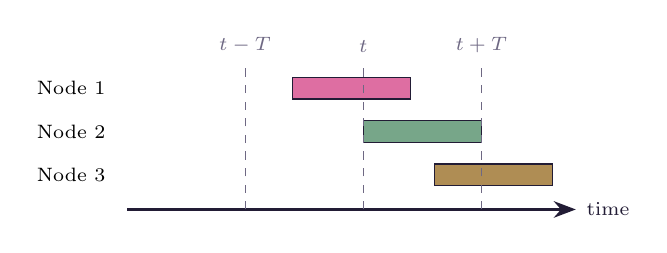
\begin{tikzpicture}[x=1.5cm,y=0.55cm,font=\scriptsize]
  \foreach \y/\n in {2/1,1/2,0/3} \node[anchor=east] at (-0.1,\y) {Node \n};
  \fill[ppink!70,draw=ink] (1.4,1.75) rectangle (2.4,2.25);
  \fill[pgreen!60,draw=ink] (2,0.75) rectangle (3,1.25);
  \fill[pgold!70,draw=ink] (2.6,-0.25) rectangle (3.6,0.25);
  \draw[arr] (0,-0.8)--(3.8,-0.8) node[right]{time};
  \draw[dashed,muted] (1,-0.8)--(1,2.6) node[above]{$t-T$};
  \draw[dashed,muted] (2,-0.8)--(2,2.6) node[above]{$t$};
  \draw[dashed,muted] (3,-0.8)--(3,2.6) node[above]{$t+T$};
\end{tikzpicture}
\figcap{After slide 29. Node 2 starts at time $t$. Node 1 started less than $T$ earlier and node 3 starts less than $T$ later: both overlap node 2's frame, so all three frames are lost.}
\end{center}

\begin{defn}[Vulnerable period]
The \term{vulnerable period} of a frame is the set of times at which \emph{another} transmission may not start, or the frame collides.
\begin{itemize}
  \item Slotted ALOHA: only the frame's own slot, length $T$.
  \item Pure ALOHA: any start in $(t-T,\,t+T)$ overlaps a frame sent at $t$, so the vulnerable period is \hl{$2T$}.
\end{itemize}
\end{defn}

\textbf{The success probability, step by step.}
\begin{enumerate}
  \item Fix a node $i$ that transmits in its own slot $[t,t+T]$: probability $p$.
  \item Any other node $j$ has its own, shifted slots. Exactly \textbf{two} of node $j$'s slots overlap $[t,t+T]$: the one that started in $(t-T,t]$ and the one that starts in $(t,t+T)$.
  \item Node $j$ stays silent in both with probability $(1-p)^2$. For all $n-1$ other nodes, by independence: $\big((1-p)^2\big)^{n-1} = (1-p)^{2(n-1)}$.
  \item So node $i$ succeeds with probability $p(1-p)^{2(n-1)}$. The success events of different nodes are disjoint, so we add over the $n$ nodes:
        \[ \boxed{\ \eta = P_{\text{suc}} = np(1-p)^{2(n-1)}\ } \]
        (The goodput step is the same as in view 1 above: $\E[T_{\text{suc}}] = T\,P_{\text{suc}}$.)
\end{enumerate}

\begin{pitfall}[Slide 30: $P(\cdot)\cap P(\cdot)$]
Slide 30 writes
\[ P_{\text{suc}} = P(\text{some node transmitted})\cap P(\text{no other node transmitted in two overlapping slots}). \]
Two problems:
\begin{itemize}
  \item $\cap$ is an operation on \emph{events}, not on numbers. The correct form is $P(A\cap B)$, which equals $P(A)P(B)$ when $A$ and $B$ are independent (the next line of the slide).
  \item ``$P(\text{some node transmitted})$'' is then set to $np$. But the probability that \emph{some} node transmits is $1-(1-p)^n$, not $np$ (for $n=10$, $p=0.2$: $0.89$, while $np = 2$, not even a probability).
        The factor $n$ really comes from \emph{adding} the $n$ disjoint events ``node $i$ transmits and all others are silent'', as in step 4.
\end{itemize}
The final formula on the slide is correct.
\end{pitfall}

\textbf{The best $p$} (slide 31 only states it). Differentiate as in the slotted case:
\[ \frac{d\eta}{dp} = n(1-p)^{2n-3}\big[(1-p) - 2(n-1)p\big] = 0\quad\Longrightarrow\quad p^* = \frac{1}{2n-1}. \]
Substituting, with $m = 2n-1$:
\[ \eta(p^*) = \frac{n}{2n-1}\Big(1-\frac1m\Big)^{m-1}\ \xrightarrow{\ n\to\infty\ }\ \frac12\cdot\frac1e = \frac1{2e}\approx0.18. \]

\begin{pitfall}[Slide 31: ``the goodput is $1/(2e)$'']
$1/(2e)$ is the goodput only in the limit of many nodes. For finite $n$ the best goodput is larger: $0.296$ for $n=2$, $0.216$ for $n=5$, $0.191$ for $n=20$ (table in Part A).
\end{pitfall}

\section{The Poisson models}\label{sec:poisson}

Slide 20 promises four models, but the recitation analyses only the two binomial ones. Here are the other two. Now infinitely many nodes start on average $G$ transmissions per slot,
so the number of starts in any interval of length $\tau$ is $\text{Poi}(G\tau/T)$ \src{BG 4.2.2}. Recall $P(\text{Poi}(\mu) = k) = e^{-\mu}\mu^k/k!$.

\textbf{Slotted, Poisson.}
\begin{enumerate}
  \item A slot succeeds iff exactly one transmission starts in it: $P(X=1) = e^{-G}G$.
  \item Goodput, as in view 1: $\eta = Ge^{-G}$.
  \item Best $G$: $\frac{d}{dG}\,Ge^{-G} = (1-G)e^{-G} = 0$, so $G^*=1$ and $\eta_{\max} = e^{-1}\approx0.37$.
\end{enumerate}

\textbf{Pure, Poisson.}
\begin{enumerate}
  \item A frame starting at $t$ succeeds iff no other frame starts in its vulnerable period of length $2T$. The number of starts there is $\text{Poi}(2G)$, so $P(\text{no other start}) = e^{-2G}$.
  \item Frames start at rate $G$ per slot, and each succeeds with probability $e^{-2G}$: $\eta = Ge^{-2G}$ \src{BG 4.2.4}.
  \item Best $G$: $(1-2G)e^{-2G} = 0$, so $G^* = \frac12$ and $\eta_{\max} = \frac12e^{-1} = \frac1{2e}\approx0.18$.
\end{enumerate}

\begin{example}[Goodput vs.\ load $G$]
\begin{center}
\renewcommand{\arraystretch}{1.2}
\begin{tabular}{>{\columncolor{border}}c c c}
\thd{$G$ (ATTEMPTS PER SLOT)} & \cellcolor{border}\thd{SLOTTED $Ge^{-G}$} & \cellcolor{border}\thd{PURE $Ge^{-2G}$}\\
\rowcolor{surface} \cellcolor{border}\color{surface}0.25 & 0.195 & 0.152\\
\rowcolor{surface2} \cellcolor{border}\color{surface}0.5 & 0.303 & \textbf{0.184}\\
\rowcolor{surface} \cellcolor{border}\color{surface}1 & \textbf{0.368} & 0.135\\
\rowcolor{surface2} \cellcolor{border}\color{surface}2 & 0.271 & 0.037\\
\end{tabular}
\end{center}
At $G=2$ the channel is overloaded: slotted ALOHA keeps $27\%$, pure ALOHA only $4\%$.
\end{example}

\begin{intuition}[The two models agree]
Put $p = G/n$ in the binomial formula: $np(1-p)^{n-1} = G(1-G/n)^{n-1}\to Ge^{-G}$ as $n\to\infty$, the same limit as in Part A's $(1-1/N)^N\to1/e$. The Poisson model is simply the binomial
model with infinitely many nodes, each very quiet. That is why both give $1/e$ and $1/(2e)$.
\end{intuition}

\begin{center}
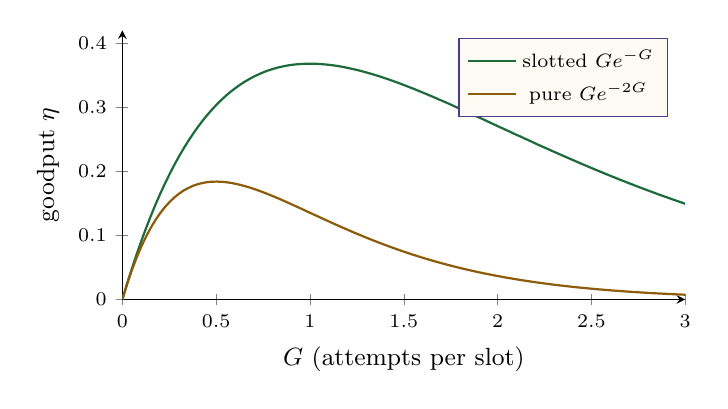
\begin{tikzpicture}
\begin{axis}[width=0.72\linewidth,height=5cm,xmin=0,xmax=3,ymin=0,ymax=0.42,
  xlabel={$G$ (attempts per slot)},ylabel={goodput $\eta$},axis lines=left,
  tick label style={font=\scriptsize},label style={font=\small},
  legend style={font=\scriptsize,draw=border,fill=surface},legend pos=north east]
  \addplot[pgreen,thick,domain=0:3,samples=120] {x*exp(-x)};
  \addplot[pgold,thick,domain=0:3,samples=120] {x*exp(-2*x)};
  \legend{slotted $Ge^{-G}$,pure $Ge^{-2G}$}
\end{axis}
\end{tikzpicture}
\figcap{Poisson models. The slotted curve peaks at $G=1$ with $1/e$, the pure one at $G=1/2$ with $1/(2e)$. Beyond the peak, more attempts mean \emph{less} goodput.}
\end{center}

\section{Question 1: one host, two networks}

\begin{center}
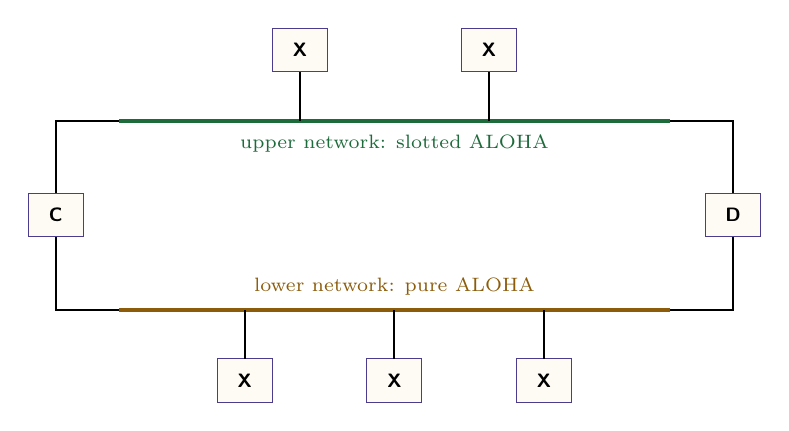
\begin{tikzpicture}[font=\scriptsize,node distance=1cm]
  \tikzset{host/.style={draw=border,fill=surface,minimum width=0.7cm,minimum height=0.55cm,font=\sffamily\bfseries\scriptsize}}
  \draw[line width=1.6pt,pgreen] (0,1.2)--(7,1.2) node[pos=0.5,below=1pt]{upper network: slotted ALOHA};
  \draw[line width=1.6pt,pgold] (0,-1.2)--(7,-1.2) node[pos=0.5,above=1pt]{lower network: pure ALOHA};
  \node[host] (C) at (-0.8,0) {C}; \node[host] (D) at (7.8,0) {D};
  \draw[thick] (C.north)|-(0,1.2); \draw[thick] (C.south)|-(0,-1.2);
  \draw[thick] (D.north)|-(7,1.2); \draw[thick] (D.south)|-(7,-1.2);
  \foreach \x in {2.3,4.7} {\node[host] at (\x,2.1) {X}; \draw[thick] (\x,1.82)--(\x,1.2);}
  \foreach \x in {1.6,3.5,5.4} {\node[host] at (\x,-2.1) {X}; \draw[thick] (\x,-1.82)--(\x,-1.2);}
\end{tikzpicture}
\figcap{After slide 32. C and D are attached to both networks. The upper network (slotted ALOHA) has two other nodes, the lower one (pure ALOHA) has three.}
\end{center}

\textbf{Setup (slide 33).} D never sends. When C has a message for D, it picks the upper network with probability $p$ (the lower one with probability $1-p$) and then sends with probability $q$.
In every slot, each X node sends with probability $q$, independently.

\subsection*{Question 1a: a single attempt}
\textbf{Question.} C has one attempt. What is the probability that the message reaches D?

\begin{enumerate}
  \item \textbf{Split by the network chosen} (law of total probability):
        \[ P^{\text{total}}_{\text{suc}} = p\cdot P^{\text{upper}}_{\text{suc}} + (1-p)\cdot P^{\text{lower}}_{\text{suc}}. \]
  \item \textbf{Upper network (slotted)}. C must send ($q$) and the two X nodes must be silent \emph{in this one slot} ($(1-q)^2$):
        \[ P^{\text{upper}}_{\text{suc}} = q(1-q)^2. \]
  \item \textbf{Lower network (pure)}. C must send ($q$), and each of the three X nodes must be silent in \emph{both} of its slots that overlap C's frame ($(1-q)^2$ each):
        \[ P^{\text{lower}}_{\text{suc}} = q\,\big((1-q)^2\big)^3 = q(1-q)^6. \]
  \item \textbf{Combine}:
        \[ \boxed{\ P^{\text{total}}_{\text{suc}} = q\big[p(1-q)^2 + (1-p)(1-q)^6\big]\ } \]
\end{enumerate}

\begin{example}[Numbers: $p=0.5$, $q=0.2$]
Upper: $0.2\cdot0.8^2 = 0.128$. Lower: $0.2\cdot0.8^6 = 0.0524$. Total: $0.5\cdot0.128+0.5\cdot0.0524 = 0.090$.
The lower network is worse for two reasons: it has one more competing node, and pure ALOHA doubles each node's vulnerable window. Each X node there counts like \emph{two} slotted nodes,
so the lower network behaves like a slotted network with six competitors.
\end{example}

\begin{pitfall}[C's own $q$]
C's chance of \emph{sending at all} is $q$, so even an empty network gives success only with probability $q$. That is why $q$ multiplies everything. The best choice of network is the upper one for every $q$, since $(1-q)^2\ge(1-q)^6$; so C should take $p=1$.
\end{pitfall}

\subsection*{Question 1b: the goodput of the upper network}
\textbf{Question.} C now tries at the beginning of every slot. What is the goodput of the upper network?


Now C is an active node like the others. In each slot it picks a network (upper with probability $p$) and sends with probability $q$. We need the probability that \emph{some} frame on the upper network succeeds.

\begin{enumerate}
  \item \textbf{C chose the upper network} (probability $p$): there are 3 active nodes (C and the two X's), each sending with probability $q$. Exactly one must send:
        \[ P^{1}_{\text{suc}} = \binom31 q(1-q)^2 = 3q(1-q)^2. \]
  \item \textbf{C chose the lower network} (probability $1-p$): only the 2 X nodes compete on the upper network:
        \[ P^{2}_{\text{suc}} = \binom21 q(1-q) = 2q(1-q). \]
  \item \textbf{Goodput} = probability of a successful slot (view 1):
        \[ \boxed{\ \eta^{\text{upper}} = p\cdot3q(1-q)^2 + (1-p)\cdot2q(1-q)\ } \]
\end{enumerate}

\begin{example}[Numbers: $p=0.5$, $q=0.2$]
$3\cdot0.2\cdot0.64 = 0.384$ and $2\cdot0.2\cdot0.8 = 0.32$, so $\eta^{\text{upper}} = 0.5\cdot0.384+0.5\cdot0.32 = 0.352$.
Compare with the slotted formula $nq(1-q)^{n-1}$: with $n=3$ nodes the best $q$ is $1/3$ (goodput $4/9 = 0.444$); with $n=2$ it is $1/2$ (goodput $0.5$). $q = 0.2$ is too timid for such a small network.
\end{example}

\begin{intuition}[Why 1b counts all nodes and 1a counts only C]
In 1a we asked whether \emph{C's} message arrives: one specific node. In 1b we ask about the \emph{network's} goodput: a slot is useful if \emph{any} single node succeeds, so we add over the nodes, hence the binomial coefficients $\binom31$ and $\binom21$.
\end{intuition}

\section{Question 2: slotted and pure nodes on one channel}

\textbf{Setup (slide 42).} There are $2n$ nodes on one channel.
\begin{itemize}
  \item Nodes $1,\dots,n$ run \textbf{pure ALOHA} with slots of length $T$ (each on its own clock).
  \item Nodes $n+1,\dots,2n$ run \textbf{slotted ALOHA} with slots of length $2T$ (synchronized among themselves).
\end{itemize}
At the beginning of each of its slots, every node sends with probability $p$, and its message fills the whole slot. So pure nodes send short frames ($T$) and slotted nodes long ones ($2T$).

\begin{center}
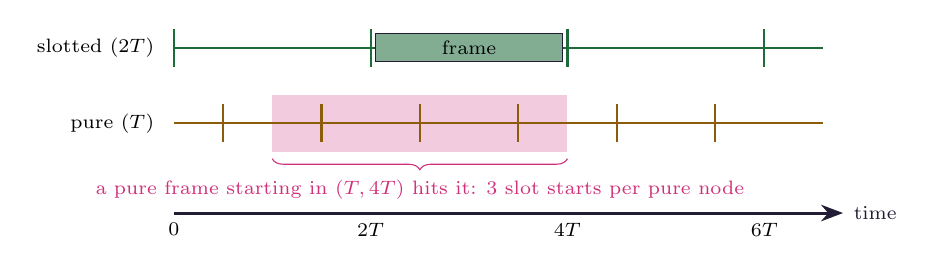
\begin{tikzpicture}[x=1.25cm,y=0.6cm,font=\scriptsize]
  \node[anchor=east] at (-0.1,1.6) {slotted ($2T$)};
  \node[anchor=east] at (-0.1,0) {pure ($T$)};
  \foreach \x in {0,2,4,6} \draw[pgreen,thick] (\x,1.2)--(\x,2.0);
  \draw[pgreen,thick] (0,1.6)--(6.6,1.6);
  \fill[pgreen!55,draw=ink] (2.05,1.3) rectangle (3.95,1.9); \node at (3,1.6) {frame};
  \fill[ppink!25] (1,-0.6) rectangle (4,0.6);
  \foreach \x in {0.5,1.5,2.5,3.5,4.5,5.5} \draw[pgold,thick] (\x,-0.4)--(\x,0.4);
  \draw[pgold,thick] (0,0)--(6.6,0);
  \draw[decorate,decoration={brace,amplitude=4pt,mirror},ppink] (1,-0.75)--(4,-0.75) node[midway,below=4pt]{a pure frame starting in $(T,4T)$ hits it: 3 slot starts per pure node};
  \draw[arr] (0,-1.9)--(6.8,-1.9) node[right]{time};
  \foreach \x/\l in {0/0,2/2T,4/4T,6/6T} \node[below] at (\x,-1.9) {$\l$};
\end{tikzpicture}
\figcap{Question 2a. A slotted node's frame occupies $[2T,4T]$. A pure node's frame of length $T$ collides with it if it starts anywhere in $(T,4T)$, an interval of length $3T$ that contains exactly three of that pure node's slot starts.}
\end{center}

\subsection*{Question 2a: a slotted node}
\textbf{Question.} In a random slot, what is the probability that a node running slotted ALOHA sends successfully?


A slotted node succeeds iff \emph{all three} of these hold (they involve different nodes, so they are independent and we multiply):
\begin{enumerate}
  \item it sends: $p$;
  \item the other $n-1$ slotted nodes do not send in this $2T$ slot: $(1-p)^{n-1}$;
  \item no pure node starts a frame in the $3T$ window of the figure. Each pure node has 3 slot starts there and must skip all three: $(1-p)^3$; for $n$ pure nodes, $(1-p)^{3n}$.
\end{enumerate}
\[ \boxed{\ P^{\text{slotted}}_{\text{suc}} = p\,(1-p)^{n-1}(1-p)^{3n}\ } \]

\begin{intuition}[Why 3 and not 2]
For two frames of the same length $T$, the vulnerable window is $2T$ (frame length plus the length of the other frame). In general it is \hl{(own length) + (other's length)}: here $2T + T = 3T$.
Long frames are especially exposed to unsynchronized short ones.
\end{intuition}

\subsection*{Question 2b: a pure node}
\textbf{Question.} In a random slot, what is the probability that a node running pure ALOHA sends successfully?


The pure node's frame has length $T$. The other pure nodes are handled as in plain pure ALOHA: $(1-p)^{2(n-1)}$. The slotted nodes depend on where the frame falls relative to the $2T$ grid. There are two cases (slides 44--46):

\begin{center}
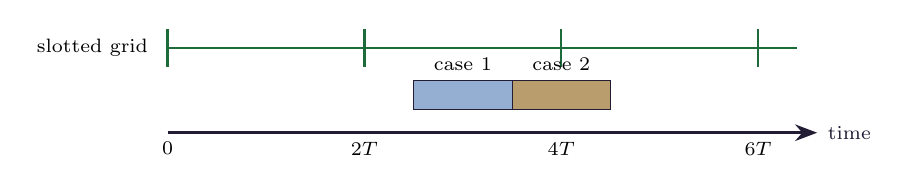
\begin{tikzpicture}[x=1.25cm,y=0.6cm,font=\scriptsize]
  \foreach \x in {0,2,4,6} \draw[pgreen,thick] (\x,0.6)--(\x,1.4);
  \draw[pgreen,thick] (0,1)--(6.4,1);
  \node[anchor=east] at (-0.1,1) {slotted grid};
  \fill[pcyan!50,draw=ink] (2.5,-0.3) rectangle (3.5,0.3); \node[above] at (3,0.3) {case 1};
  \fill[pgold!60,draw=ink] (3.5,-0.3) rectangle (4.5,0.3); \node[above] at (4,0.3) {case 2};
  \draw[arr] (0,-0.8)--(6.6,-0.8) node[right]{time};
  \foreach \x/\l in {0/0,2/2T,4/4T,6/6T} \node[below] at (\x,-0.8) {$\l$};
\end{tikzpicture}
\figcap{Case 1: the pure frame lies inside one $2T$ slot. Case 2: it straddles the boundary between two $2T$ slots.}
\end{center}

\textbf{Case 1, inside one $2T$ slot}: no slotted node may send in that one slot, $(1-p)^n$:
\[ P_1 = p\,(1-p)^n(1-p)^{2(n-1)}. \]
\textbf{Case 2, straddling two $2T$ slots}: no slotted node may send in either, $(1-p)^{2n}$:
\[ P_2 = p\,(1-p)^{2n}(1-p)^{2(n-1)}. \]

\textbf{Combining the cases} (the slides stop before this). Shift the pure node's slots by any offset $0<\varphi<T$ against the $2T$ grid: its slots then alternate between case 1 and case 2. So \hl{exactly half} of its slots are of each kind, and a random slot gives
\[ \boxed{\ P^{\text{pure}}_{\text{suc}} = \tfrac12P_1 + \tfrac12P_2 = \tfrac12\,p\,(1-p)^{2(n-1)}\big[(1-p)^n + (1-p)^{2n}\big]\ } \]

\begin{example}[Numbers: $n=5$, $p=0.1$]
Slotted node (2a): $0.1\cdot0.9^4\cdot0.9^{15} = 0.0135$. Pure node (2b): $P_1 = 0.1\cdot0.9^5\cdot0.9^8 = 0.0254$, $P_2 = 0.1\cdot0.9^{10}\cdot0.9^8 = 0.0150$, average $0.0202$.
A pure node succeeds more often than a slotted one: its short frame has a smaller vulnerable window.
\end{example}

\subsection*{Question 2c: everybody synchronized}
\textbf{Question.} The pure nodes switch to slotted ALOHA with slots of length $T$, synchronized with the $2T$ slots. What is the goodput of the network?


Now every $2T$ slot of the long-frame nodes is split into two aligned $T$ slots of the short-frame nodes. Look at one $2T$ window. Write
\[ s = np(1-p)^{n-1}\ \ (\text{exactly one of $n$ nodes sends}),\qquad z = (1-p)^n\ \ (\text{none of $n$ nodes sends}). \]
The window can contain these successful outcomes (slides 47--49):
\begin{center}
\renewcommand{\arraystretch}{1.3}
\begin{tabular}{>{\columncolor{border}}c p{6.2cm} c c}
\thd{} & \cellcolor{border}\thd{OUTCOME} & \cellcolor{border}\thd{PROBABILITY} & \cellcolor{border}\thd{USEFUL TIME}\\
\rowcolor{surface} \cellcolor{border}\color{surface}A & one long frame succeeds: exactly one long node sends, no short node sends in either half & $s\,z^2$ & $2T$\\
\rowcolor{surface2} \cellcolor{border}\color{surface}B & short success in the first half only: no long node sends, exactly one short node in half 1, not exactly one in half 2 & $s\,z\,(1-s)$ & $T$\\
\rowcolor{surface} \cellcolor{border}\color{surface}C & short success in the second half only (same as B) & $s\,z\,(1-s)$ & $T$\\
\rowcolor{surface2} \cellcolor{border}\color{surface}D & short successes in both halves: no long node, exactly one short node in each half & $s^2z$ & $2T$\\
\end{tabular}
\end{center}
Dividing useful time by $2T$ gives the slide's answer:
\[ \eta = A + \tfrac12B + \tfrac12C + D. \]

\textbf{Simplifying.} Substitute and collect: $\eta = sz^2 + sz(1-s) + s^2z = sz^2 + sz$, so
\[ \boxed{\ \eta = s\,z\,(1+z) = np(1-p)^{2n-1}\big(1+(1-p)^n\big)\ } \]

\begin{intuition}[A shortcut: linearity of expectation]
We can skip the four cases. Useful time in the window = (useful time from long frames) + (useful time in half 1) + (useful time in half 2), and \emph{expectations add even when the parts are dependent}.
\begin{itemize}
  \item Long: $2T$ with probability $sz^2$, i.e.\ a fraction $sz^2$ of the window.
  \item Each half: $T$ with probability $sz$ (exactly one short node, no long node), i.e.\ $\frac12sz$ of the window per half.
\end{itemize}
Total: $sz^2 + 2\cdot\frac12sz = sz(1+z)$. Same answer, no case analysis.
\end{intuition}

\begin{example}[Did synchronizing help? $n=5$, $p=0.1$]
\textbf{After} (2c): $s = 5\cdot0.1\cdot0.9^4 = 0.328$, $z = 0.9^5 = 0.590$, so $\eta = 0.328\cdot0.590\cdot1.590 = 0.308$.\\
\textbf{Before} (2a, 2b): per $2T$ window, the $n$ long nodes deliver on average $n\cdot P^{\text{slotted}}_{\text{suc}}\cdot2T$ and the $n$ short nodes, each with 2 slots, $n\cdot2\cdot P^{\text{pure}}_{\text{suc}}\cdot T$. Dividing by $2T$:
$\eta = n\,P^{\text{slotted}}_{\text{suc}} + n\,P^{\text{pure}}_{\text{suc}} = 5\cdot0.0135 + 5\cdot0.0202 = 0.169$.\\
Aligning the short nodes' slots nearly \hl{doubles} the goodput, the same factor of 2 as between pure and slotted ALOHA. Optimizing $p$ for $n=100$ (numerically): about $0.20$ before and $0.30$ after.
Even after, the mixed network stays below $1/e$: a long frame needs \emph{both} halves free of short frames.
\end{example}

% =================================================================
\parttitle{WEEK 02}{Practice Problems and Summary}
% =================================================================

\section{Practice problems with full solutions}

\begin{example}[P1: Layers]
A router receives an Ethernet frame and forwards the packet on a SONET link. Which headers does it read, and which does it replace?

\textbf{Solution.} It removes the Ethernet (link) header, reads the IP (network) header to choose the outgoing link, decrements the TTL, and wraps the datagram in a new
SONET link header. It never reads the TCP or HTTP headers: transport and application exist only at the hosts.
\end{example}

\begin{example}[P2: Encapsulation overhead]
An application sends 100 bytes over TCP/IP/Ethernet. What fraction of the frame (headers only) is data? And for 1000 bytes?

\textbf{Solution.} $100/154=64.9\%$. $1000/1054=94.9\%$.
\end{example}

\begin{example}[P3: Slotted ALOHA]
$N=4$ nodes, each transmits in a slot with probability $p=0.2$. (a) Probability that node 1 succeeds in a slot? (b) Goodput? (c) The best $p$ and its goodput?

\textbf{Solution.} (a) $0.2\cdot0.8^3=0.1024$. (b) $4\times0.1024=0.4096$. (c) $p^*=1/4$: $(3/4)^3=0.4219$.
\end{example}

\begin{example}[P4: Empty slots]
In P3 with $p=0.2$, what fraction of slots is empty, and what fraction has collisions?

\textbf{Solution.} Empty: $0.8^4=0.4096$. Collisions: $1-0.4096-0.4096=0.1808$.
\end{example}

\begin{example}[P5: Pure ALOHA]
$N=3$ nodes, $p=0.2$. Goodput of pure ALOHA? Compare with slotted ALOHA.

\textbf{Solution.} Pure: $3\cdot0.2\cdot0.8^{4}=0.2458$. Slotted: $3\cdot0.2\cdot0.8^{2}=0.384$. Pure is lower because the vulnerable window is twice as long.
\end{example}

\begin{example}[P6: CSMA/CD minimum frame]
A CSMA/CD LAN runs at 100\,Mbps over at most 200\,m of cable ($s=2\times10^8$\,m/s). What is the minimum frame size?

\textbf{Solution.} $\PROP=200/(2\times10^8)=1\,\mu$s. Need $\TRANSP\ge2\,\PROP=2\,\mu$s, so $L\ge2\times10^{-6}\times10^8=200$ bits $=25$ bytes.
\end{example}

\begin{example}[P7: CSMA/CD efficiency]
$\PROP=5\,\mu$s and $\TRANSP=100\,\mu$s. Find $a$ and the efficiency in both models.

\textbf{Solution.} $a=0.05$. Simple model: $1/(1+0.15)=87\%$. Simulation model: $1/(1+0.25)=80\%$.
\end{example}

\begin{example}[P8: Wasted slots]
In the CSMA/CD model, a slot is won with probability $\alpha=0.25$. Expected wasted slots per packet?

\textbf{Solution.} $A=(1-\alpha)/\alpha=0.75/0.25=3$ slots, i.e.\ $3\times2\,\PROP=6\,\PROP$ of overhead per packet.
\end{example}

\begin{example}[P9: Exponential backoff]
Two Ethernet NICs collide for the 3rd time on a 10\,Mbps LAN. (a) From which set is $K$ chosen? (b) Probability that they collide again? (c) Longest possible wait?

\textbf{Solution.} (a) $\{0,\dots,7\}$. (b) They pick the same $K$ with probability $8\cdot(1/8)^2=1/8$. (c) $7\times512\times0.1\,\mu$s $=358.4\,\mu$s.
\end{example}

\begin{example}[P10: Hidden terminal]
A, B and C are in a line; A and C are each 80\,m from B, and the radio range is 100\,m. Can A and C hear each other? Which mechanism stops their data frames from colliding at B?

\textbf{Solution.} A and C are 160\,m apart, beyond the range: they are hidden from each other, so carrier sensing fails. RTS/CTS: B's CTS reaches both, so the station that did not win the CTS defers.
\end{example}

\subsection*{Recitation problems}

\begin{example}[P11: Goodput in bits per second]
A slotted ALOHA channel has $B = 1$\,Mbps and frames of $L = 1000$ bits. There are 4 nodes with $p = 0.25$. (a) Slot length? (b) Goodput? (c) Useful bit rate? (d) Average time between successful frames?

\textbf{Solution.} (a) $T = L/B = 1$\,ms. (b) $\eta = 4\cdot0.25\cdot0.75^3 = 0.422$. (c) $0.422\times1$\,Mbps $=422$\,kbps. (d) View 2: $T/\eta = 1/0.422 = 2.37$\,ms.
\end{example}

\begin{example}[P12: Which layer?]
Place in the OSI model: TLS encryption, TCP acknowledgements, Ethernet's binary exponential backoff, choosing a route between two cities.

\textbf{Solution.} TLS: presentation (6) in OSI; in the Internet stack the application provides it. TCP ACKs: transport (4). Backoff: data link (2), MAC sub-layer. Routing: network (3).
\end{example}

\begin{example}[P13: Poisson load]
A slotted ALOHA channel carries on average $G = 0.6$ attempts per slot. (a) Fraction of slots that are successful, empty and collisions? (b) Same load on pure ALOHA?

\textbf{Solution.} (a) Success $0.6e^{-0.6} = 0.329$; empty $e^{-0.6} = 0.549$; collision $1-0.329-0.549 = 0.122$. (b) $0.6e^{-1.2} = 0.181$, almost exactly the pure maximum $1/(2e)=0.184$, because $G=0.6$ is close to $G^*=0.5$.
\end{example}

\begin{example}[P14: Question 1 variant]
In Question 1, let the lower network also run \emph{slotted} ALOHA. With $p=0.5$, $q=0.2$, what is C's one-shot success probability now?

\textbf{Solution.} Lower: $q(1-q)^3 = 0.2\cdot0.512 = 0.1024$. Total: $0.5\cdot0.128 + 0.5\cdot0.1024 = 0.115$, up from $0.090$: synchronizing the lower network halves each X node's vulnerable window.
\end{example}

\begin{example}[P15: Vulnerable windows of mixed lengths]
A pure ALOHA channel carries frames of length $T$ and of length $3T$. How long is the vulnerable window of a $3T$ frame against $T$ frames, and of a $T$ frame against $3T$ frames?

\textbf{Solution.} (Own length) + (other's length) in both cases: $3T + T = 4T$. The window is the same, but a long frame occupies more of the channel each time it collides.
\end{example}

\begin{example}[P16: Question 2c with numbers]
In Question 2c, take $n = 10$, $p = 0.05$. Find $\eta$.

\textbf{Solution.} $s = 10\cdot0.05\cdot0.95^9 = 0.315$, $z = 0.95^{10} = 0.599$. $\eta = sz(1+z) = 0.315\cdot0.599\cdot1.599 = 0.302$.
\end{example}

\section{Cheat sheet}

\begin{formula}[Week 02 on one page]
\begin{itemize}
  \item Modularity: interfaces hide implementation; extensible; can cost performance. Network design choices: layering, where to implement, where to keep state.
  \item Layers: Physical (bits) / Link (frames, local addresses, MAC) / Network (packets, global addresses, routing, IP only) / Transport (processes; TCP, UDP) / Application. Routers: bottom 3. Hosts: all 5.
  \item Protocol = syntax (format, order) + semantics (meaning, actions). Standards: IETF RFCs. Layer = service + interface + protocol.
  \item Encapsulation: each layer adds a header. TCP 20 + IP 20 + Ethernet 14 = 54 bytes. Hourglass: IP is the narrow \emph{waist}.
  \item MAC protocol: distributed; coordinates over the channel itself. Wish list: alone $\to R$; $M$ busy $\to R/M$; decentralized; no sync; simple.
  \item TDMA/FDMA: no collisions, fair, but $R/N$ even when alone; unused slots/bands idle.
  \item Slotted ALOHA: $\alpha=Np(1-p)^{N-1}$, $p^*=1/N$, max $(1-\frac1N)^{N-1}\to1/e\approx0.37$. Pure ALOHA: $Np(1-p)^{2(N-1)}$, max $\to1/(2e)\approx0.18$.
  \item CSMA: listen first; collisions still happen because of propagation delay. CSMA/CD: abort on collision; need $\TRANSP\ge2\,\PROP$.
  \item CSMA/CD goodput: $A=(1-\alpha)/\alpha$; $\eta=1/(1+3a)$ (simple), $\approx1/(1+5a)$ (precise), $a=\PROP/\TRANSP$.
  \item Ethernet: after the $m$-th collision $K\in\{0,\dots,2^m-1\}$ (capped at $m=10$), wait $K\cdot512$ bit times; jam 48 bits; bit time $0.1\,\mu$s at 10\,Mbps.
  \item MAC address: 48 bits, flat, portable, IEEE gives 24-bit prefixes. IP address: hierarchical, not portable.
  \item 802.11: no CD (weak received signal, hidden terminal, fading) $\Rightarrow$ CSMA/CA: DIFS, random backoff frozen while busy, ACK after SIFS; RTS/CTS reserves the channel.
\end{itemize}
\end{formula}

\begin{formula}[Recitation 2 on one page]
\begin{itemize}
  \item OSI: Physical (bit) / Data link (frame) / Network (packet) / Transport (segment) / Session / Presentation / Application. Internet: layers 5--7 merged into the application. Wi-Fi and Ethernet are layers 1 \emph{and} 2; MAC is a sub-layer of 2.
  \item $T = L/B$. Throughput: fraction of time anything is sent. Goodput $\eta$: fraction of time spent on \emph{successful} sends. $\times B$ gives bits/s.
  \item Two views: $\eta = \E[T_{\text{suc}}]/T = P_{\text{suc}}$ (one slot), or $T/(T\cdot\E[\text{Geo}(P_{\text{suc}})]) = P_{\text{suc}}$ (wait for success).
  \item Binomial: slotted $np(1-p)^{n-1}$, $p^*=1/n$, $\to1/e$. Pure $np(1-p)^{2(n-1)}$, $p^*=1/(2n-1)$, $\to1/(2e)$.
  \item Poisson ($G$ attempts per slot): slotted $Ge^{-G}$, max $1/e$ at $G=1$; pure $Ge^{-2G}$, max $1/(2e)$ at $G=\frac12$. Binomial with $p=G/n$, $n\to\infty$.
  \item Vulnerable window (pure) = own frame length + other frame length: $2T$ for equal frames.
  \item Pure node vs.\ slotted grid of $2T$: half its frames inside one slot, half straddling two.
  \item Exam tricks: split by cases with total probability; ``one specific node'' $\to$ no $\binom n1$, ``any node'' $\to$ multiply by $n$; use linearity of expectation to avoid case analysis.
\end{itemize}
\end{formula}

\end{document}
